\documentclass[twocolumn]{aastex631}
\bibliographystyle{aasjournal}
\usepackage{amsmath}
\usepackage{amssymb}
\usepackage{amsfonts}
\usepackage{mathtools}
\usepackage{url}
\usepackage{booktabs} 

\newcommand{\done}{{\tt d1}}
\newcommand{\dnine}{{\tt d9}}

\usepackage{color}
\newcommand{\bsh}[1]{\textcolor{red}{(BSH: #1)}}
\newcommand{\giuse}[1]{\textcolor{orange}{(GP: #1)}}
\newcommand{\sg}[1]{\textcolor{teal}{(SG: #1)}}
\newcommand{\mr}[1]{\textcolor{magenta}{#1}}
\providecommand{\sorthelp}[1]{}

\begin{document}

\title{The Python Sky Model 3.1: \\Improved Models of Galactic Dust and Synchrotron Emission}
\author{PanEx PySM Team}
\date{\today}

\begin{abstract}
    Lorem ipsum
\end{abstract}

\section{Introduction}
%writing: Brandon, Julian (multi-experiment collab), Susan + others

One of the principal challenges for current and future cosmic microwave background (CMB) polarization experiments is mitigating contaminating emission from the Galaxy. Polarized Galactic emission is brighter than current upper limits on a primordial B-mode signal at all frequencies, even in particularly clean patches of high Galactic latitude sky, while future surveys targeting wide areas ($f_{\rm sky} \gtrsim 50\%$ for cosmological analyses) will measure polarized Galactic emission more than an order of magnitude brighter. Thus understanding the potential complexities of Galactic emission and designing analyses robust to them is of paramount importance for constraining the physics of the early Universe.

To this end, tools have been developed to simulate full-sky, multi-frequency realizations of Galactic emission drawing both on data-driven constraints and theoretical models. The Planck Sky Model \citep[PSM;][]{delabrouille2012} was originally put together to develop data analysis tools for the Planck mission, using pre-existing data sets. It evolved throughout the Planck mission timeline to gradually include Planck observations and adjust to Planck data analysis requirements, and has been widely used in various data challenges and/or for planning future CMB experiments \textcolor{red}{[JD: Should we cite a few examples here, or leave it at that?]}. Building on the PSM, the Python Sky Model \citep[PySM;][]{Thorne:2017} provides a Pythonic interface to expanded classes of foreground models. PySM has been widely used for both data analysis and forecasting \citep[e.g.,][]{CCAT-Primecollaboration:2021,Hensley:2021}. %As the sensitivity of CMB experiments is improved, 

In this work, we introduce several important improvements to the PySM software. First, we update foreground emission templates at large angular scales to agree with current best determinations. Second, we develop and implement a new framework for simulating stochastic realizations of small-scale emission, allowing users to generate many realizations of the Galactic microwave sky with the same statistical properties but different small-scale morphologies. We employ this framework to include small scale fluctuations in maps of both foreground amplitudes as well as spectral parameters, such as dust temperature. Third, we implement the ``layer model'' of \citet{Martinez-Solaeche:2018} (henceforth the ``MKD'' model) in which dust emission is modeled from the sum of up to six discrete layers along the line of sight. This results in sky simulations having non-zero line-of-sight decorrelation, a phenomenon recently detected in Planck data in which the dust polarization angle can change with frequency \citep{Pelgrims:2021}. 

The models developed here follow several general principles, in line with the ethos of previous generations of Galactic emission models. The models are explicitly data-based on scales and frequencies where the Galactic emission is well-measured: we use the best available data to the extent possible. Where we do not have high-fidelity measurements, we have some freedom on the ultimate characteristics of our synthetic Galactic emission. We strive to be guided by two principles: first, we take a ``physics-first" approach to the problem wherever possible, preferring to be guided by our current understanding of ISM physics. 

% [maybe Gauss-Legendre]

We define three sets of Galactic foreground models that are both driven by the existing data where they are unambiguous and span a range of complexities (labeled low, medium, and high) in their approach to modeling emission in the parameter space where it is not well-constrained by data. This suite will enable individual experiments to optimize their designs over our current understanding of the Galactic foreground sky, and will also support comparative and especially combined analyses of multiple experiments. 
%, for example analyzing CMB-S4 data together with that of the precursor South Pole and/or Simons Observatories, or using CMB-S4 high resolution data to help delens LiteBIRD and LiteBIRD high frequency data to help remove dust from CMB-S4.

We organize the paper as follows: in Section~\ref{sec:methods}, we give an overview of how Galactic emission models are implemented in PySM; in Section~\ref{sec:templates}, we describe the new data-driven templates used to model emission at large angular scales; in Section~\ref{sec:small_scales}, we present our methodology for generating stochastic simulations of small-scale emission using the polarization fraction tensor formalism; in Section~\ref{sec:layers}, we describe the implementation of the MKD model in PySM; in Section~\ref{sec:validation}, we present a collection of validation metrics for the new models; in Section \ref{sec:modelsuite}, we present our proposed triplet of models that span a range of complexity; in Section~\ref{sec:discussion}, we discuss current limitations and future directions for development; and we conclude in Section~\ref{sec:summary}.

\section{Methods Overview} \label{sec:methods}
% writing: Andrea + others

\begin{enumerate}
    \item Recap of PySM code at more technical level than Introduction: objectives, methods
    \item Motivate aims of this paper: improved templates, generating small scales on the fly, and incorporating 3D effects
\end{enumerate}

\textbf{Andrea: technical details about PySM 3}

The groundwork that allowed the implementation of this new generation of Galactic models started in 2019 with the rewrite of PySM and its release as PySM~3 \citep[see][for details]{Zonca:2021}.

The most stringent requirement of models at high resolution is the sheer size of the templates: maps at a pixel size of 0.4 arcminutes ($N_{side}=8192$) occupy ~3\,GB per component in single precision and are 256 times larger than the original PySM~2 maps. The problem of distribution has been solved by hosting all the input templates at NERSC \footnote{\url{https://portal.nersc.gov/project/cmb/pysm-data}}, with templates downloaded and cached by PySM as needed using the facilities included in \texttt{astropy.data} \citep{AstropyCollaboration:2013, AstropyCollaboration:2018}. Moreover, all the members of the CMB community using NERSC for computing are able to directly access the same folders locally. The second issue is memory usage, PySM 3 leverages \texttt{numba} \citep{numba:2015} to compile Python on-the-fly to machine code so that the evaluation and bandpass integration of each model avoids the temporary arrays allocated by \texttt{numpy} and reduces memory consumption at least by a factor of two. Moreover, \texttt{numba} supports multi-threading so it can make use of all the cores available in the system.

Thanks to the above-mentioned improvements, we were able to create foreground models with a resolution up to $N_{side}=8192$ keeping the disk, memory and CPU requirements manageable. 

{\bf needs some motivational text on improvements, especially stochasticity but also templates}

\section{Galactic Emission Templates} \label{sec:templates}
On large angular scales, Galactic emission is well constrained at some frequencies by current data, and the models developed here should accord with these constraints as closely as possible. In this section, we describe the data-driven templates used in the new models and comment on differences with previous PySM models.

\subsection{The multicomponent ISM emission}

The Galactic interstellar medium (ISM) consists of matter and radiation in various forms. At the microwave wavelengths relevant for CMB observation, hot cosmic ray electrons spiraling in the Galactic magnetic field emit synchrotron radiation, while warm ionised gas emits free-free (or \emph{Brehmstrahlung}) radiation through the interaction of free electrons with ionized atoms. Both of those dominate the ISM emission at frequencies below $\sim$10-100~GHz, depending on the region being considered.  
Cold ($\sim$10-30~K) grains of interstellar dust primarily emit thermal radiation with a spectrum that peaks at about 2~THz, and shows an excess above a typical blackbody curve below $\nu=100$~GHz, dubbed anomalous microwave emission (AME). AME, first detected as a component of microwave emission correlated to IRAS dust maps \citep{1996ApJ...464L...5K,1997ApJ...486L..23L} and further characterized using WMAP and Planck data \citep{planck2011-7.2}, is thought to be due to spinning dust grains. Finally, atoms and molecules in the Galactic ISM, through vibrational and rotational shifts in energy levels, emit radiation in the form of a rich spectrum of discrete transition lines, including a bright comb of emission at multiples of the CO J=1-0 $\nu \simeq 115$~GHz rotational line of carbon monoxide. Here we describe our approach to modeling each of these components. 

In each sky pixel $p$, synchrotron emission $A_s(\nu,p)$ as a function of frequency is well fit by a power law with a pixel-dependent spectral index $\beta_s(p)$:
\begin{equation}
    A_s(\nu,p) \propto \nu^{\beta_s}(p),
\end{equation}
where $\beta_s(p) \simeq -3$ when the emission is expressed in Rayleigh-Jeans temperature units, and $\beta_s(p) \simeq -1$ when the emission is expressed in brightness units. Thermal dust emission $A_d(\nu,p)$ scales with frequency as
\begin{equation}
    A_d(\nu,p) \propto \nu^{\beta_d}(p) \, B_\nu(T_d(p)),
    \label{eq:dust-emission-law}
\end{equation}
where $\beta_d(p) \simeq 1.6$ on average, ranging from about 1.0 to about 2.2, and $T_d(p)$ ranges from 10 to 30~K.

\subsection{Dust Amplitude}\label{sec:dustamplitude}
The Planck~2015 component separation results in total intensity remain state of the art despite updates in polarization in the 2018 data release \citep{planck2016-l04}. Previous PySM models like \bsh{fill} employed the dust templates from the \texttt{Commander} component separation analysis \citep{planck2014-a11}. However, the model fitting employed in \citet{planck2014-a11} did not differentiate between Galactic dust emission and the Cosmic Infrared Background (CIB), and so the component separated dust maps retain CIB signal that should not be included in simulations of Galactic emission (see Section~\ref{sec:CIBcontamination} for detailed discussion).

To address this issue, we instead use dust templates for the {\tt d9} and {\tt d10} models from analyses that separated Galactic dust emission from the CIB using the Generalized Needlet Internal Linear Combination (GNILC) algorithm \citep{2011MNRAS.418..467R}. In total intensity we employ the Planck GNILC 2015 component separated map at $353$\,GHz \citep{planck2016-XLVIII}\footnote{\texttt{COM\_CompMap\_Dust-GNILC-F353\_2048\_R2.00.fits}}, 
%which has a uniform angular resolution of $28^\prime$ and pixellated with $N_{\rm side} =2048$. 
\mr{which we reprocess to have spatially uniform angular resolution. Although the original template has variable angular resolution, ranging from $21.8'$ up to $5'$ depending on the sky regions, it was synthetized from ten needlet (wavelet) maps of different, but spatially-uniform, resolution  \citep[][Figure~A.2]{planck2016-l04}. Hence, by conserving only the first six needlet maps, which probe the dust intensity from the largest scales down to $21.8'$, for the synthesis of the dust template in every pixel, we reproduced the Planck GNILC 2015 dust intensity template at $N_{\rm side} =2048$ but with a uniform $21.8'$ angular resolution all over the sky. Smaller angular scales are not reliable enough in current Planck dust templates, hence they are left for stochastic realizations [MR: \textit{Giuseppe, please confirm if this was the reason for requesting uniform resolution}].
In addition,} we subtract the CIB monopole of $0.13\, \text{MJy}\cdot\text{sr}^{-1}$ present in the map \citep[][Section~2.2]{planck2016-l04}.

For the dust $Q$ and $U$ maps we employ the dust maps\footnote{\texttt{COM\_CompMap\_IQU-thermaldust-gnilc-varres\_2048\_R3.00.fits}} produced by the GNILC component separation from the third Planck release \citep{planck2016-l04,planck2016-l11B}. These maps have a spatially varying resolution, ranging from $21.8^\prime$ in the Galactic plane to $80^\prime$ at high Galactic latitudes, and are pixellated at $N_{\rm side} = 2048$. 

% To avoid issues related to the multi-resolution nature of the $Q$ and $U$ maps, we employ the full resolution templates, including also the small angular scales, in the region around the Galactic Plane ($f_{sky}\sim 90 \%$). This region is sufficiently bright that even the small scales are measured with high signal-to-noise.

To produce dust emission templates at the monochromatic frequency of 353\,GHz, we divide each of the $I$, $Q$, and $U$ maps by a factor of 1.098 to correct for the Planck bandpass \citep[][Table~2]{planck2016-l11A}.
%Given that the intensity template has been estimated in a different way to the Q and U templates, we employ two different multipole scale cut-offs: $\ell=400$ and $100$, respectively. This further prevents the mixing of scales due to variable resolutions. 

%Moreover, the synthesis of small scales involves regions far from the Galactic plane, essentially outside in a region encoding 97\% of the sky. This is because, inside this area, the dust signal presents a very high SNR that small angular scales (e.g. $\sim20 $ arcmin ) are less affected by noise. We therefore decide to optimally exploit the state-of-art data on dust emission by employing the real small scales from observations nearby the Galactic plane. 


\subsection{Dust Spectral Parameters}
We employ the publicly available spectral parameter maps of $\beta_d$\footnote {\texttt{COM\_CompMap\_Dust-GNILC-Model-Spectral-Index\_2048\_R2.00.fits}} and $T_d$\footnote{\texttt{COM\_CompMap\_Dust-GNILC-Model-Temperature\_2048\_R2.00.fits}} derived from 2015 Planck GNILC release. These maps benefit of lower CIB residuals as the methodology employed all the Planck  high frequency channels from 100 to 857\,GHz to improve the characterization of dust intensity by means of different spectral and spatial dependence of Galactic and extra-galactic emission. However, the estimate of $\beta_d$ and $T_d$ is highly degenerate making the maps at small angular scales ($<21.8^\prime$) are contaminated by artifacts due to noise and calibration errors. The chosen cut-off multipole for $\beta_d$ and $T_d$ is the same as the one adopted for the intensity amplitude template, i.e. $\ell=400 $.  

\subsection{Synchrotron Amplitude}
% The state-of-art on  synchrotron templates is  worse than the dust ones. Although several improvements have been obtained at low frequencies, e.g. SPASS survey at 2.3 GHz, and several other surveys are expected to release soon synchrotron maps observing  both  Northern and Southern sky  (e.g. QUIJOTE CBASS),   to date a full sky map at high SNR is yet to  be produced.  

We  adopted as  intensity synchrotron template the   Haslam map  rescaled to 23 GHZ assuming a constant spectral index of -3.1. Vice versa,  Q and U templates are derived from the WMAP K-band. Both $I$ and $QU$ templates are further convolved to a  2 deg beam to further reduce the noise contamination especially in the polarization templates. Finally, we  adopt $\ell = 36$ as  cut-off multipole scale  for synchrotron.  

\subsection{Synchrotron Spectral Parameters}
To build the large scale template for the spatial variation of the synchrotron spectral index $\beta_s$, we employ the full-sky $\beta_s$ map obtained by combining the Haslam map in total intensity at 408\,MHz \citep{Remazeilles:2014} and WMAP K-band data \citep{mivilledeschenes:2008}. This $\beta_s$ map has an angular resolution of about $7^{\circ}$ and is the same employed by previous PySM synchrotron models \citep{Thorne:2017}. 

Taking advantage of the new information about synchrotron emission coming from Planck and S-PASS \citet{Krachmalnicoff:2018}, observations we modified this template in order to get as close as possible to the constraints on $\beta_s$ coming from data.
 
We further include a \emph{curvature}, $c_s$,  of the  $\beta_s$, as an extra spatially varying synchrotron parameter. The existing \texttt{s3} model  implements curvature as a single global parameter, $c_s = -0.052 $, consistent with the measurements from ARCADE \citep[$c_s=-0.052 \pm 0.005$][]{Kogut:2012}. We employed the Haslam map $I_{408}$ smoothed at 5 deg rescaled on an  appropriate range so that $c_s$ matches the \citet{Kogut:2012} measurements within the ARCADE region; the mean and standard deviation of $c_s$ template are respectively $-0.0517$ and $0.0054$. 

Finally, both the $\beta_s$ and the $c_s$ templates are low pass filtered with $\ell=36$ to minimize artifacts from noise and the large beamsize.
% Moreover,  we also add stochastic gaussian small scales to this large scale template, as described in Section~\ref{sec:beta_s}.

\subsection{CO Emission}

\subsection{AME and free-free}
\section{Stochastic Emission at Small Angular Scales} \label{sec:small_scales} 

% Susan editing/commenting 4/19
\subsection{Methodology}\label{subsec:methodology}
The methods presented here aim to preserve the well-measured large-scale information in our various templates, filter out the noisy small-scale emission in those templates, and replace those small scales with a stochastic realization that has a reasonable correspondence with the large scale emission. Specifically, the synthetic small-scale structure should have a power spectrum that connects smoothly to the power spectrum of the real data at large scales and should inherit some of the amplitude information from the large-scale data. Our approach is to construct small-scale stochastic templates and then modulate them with the large-scale amplitude data.

Rather than $I$, $Q$, and $U$, we choose to work with their analogues in the polarization fraction tensor framework (Frolov et al., in prep.). This provides a physically-motivated way to couple intensity and polarization self-consistently, and the nature of the logarithmic transformations introduces some non-Gaussianity into the final maps {\bf [see Section X]}. The transformations from $I$, $Q$, and $U$ to $i$, $q$, and $u$, respectively, are

\begin{align}
    i &\equiv \frac{1}{2} \ln (I^2 - P^2)\nonumber  \\
    q &\equiv  \frac{Q}{2P} \ln \frac{I+P}{I-P} \label{eq:pt2real}\\
    u &\equiv  \frac{U}{2P} \ln \frac{I+P}{I-P}\nonumber 
    ~~~,
\end{align}
where $P \equiv \sqrt{Q^2 + U^2}$.

The inverse transformations are:

\begin{align}
    I &= e^i \cosh p \nonumber \\
    Q &= \frac{q}{p}e^i\sinh p \label{eq:real2pt} \\
    U &= \frac{u}{p}e^i\sinh p \nonumber
    ~~~,\label{eq:real2pt}
\end{align}
where $p \equiv \sqrt{q^2 + u^2}$.

The method for generating small-scale emission can be summarized as follows: 
\begin{enumerate}
    \item We first transform the $I$, $Q$, and $U$ templates into the $i$, $q$, and $u$ maps via Equation~\eqref{eq:real2pt}. 
    \item We then compute the $tt$, $te$, $ee$, and $bb$ full-sky power spectra from the $i$, $q$, and $u$ maps in analogy with how $TT$, $TE$, $EE$, and $BB$ spectra are computed from $I$, $Q$, and $U$ maps. 
    \item We construct a simple model for each of the $tt$, $te$, $ee$, and $bb$ spectra by first estimating the amplitude of each power spectrum $A_{\ell, 1}$ at some pivot scale $\ell_1$ by fitting it with a power-law of fixed index, taken from the literature. We adopt the input templates as-is for $\ell < \ell_1$, extrapolate the spectrum with this power law from $\ell_1$ until a second pivot scale $\ell_2$, and then finally extrapolate to $\ell > \ell_2$ with the power law index of the $tt$ spectrum.
    \item We construct modulation maps $m_I$ and $m_P$ for intensity and polarization, respectively, following the methods in Section~\ref{subsec:modulation}.
    \item We then synthesize $i$, $q$, and $u$ maps using the constructed $tt$, $te$, $ee$, and $bb$ spectra. These maps are then high-pass filtered at cut-off multipole $\ell_1$ and multiplied by the modulation maps. 
    \item We low-pass filter the template $i$, $q$, and $u$ maps with cut-off multipole $\ell_1$. 
    \item Finally, we sum the small-scale and large-scale maps and then transform back to $I$, $Q$, and $U$ maps via Equation~\eqref{eq:pt2real}. 
\end{enumerate}

This prescription has several free parameters that require tuning. The pivot scale $\ell_1$ governs to which multipole information is taken from the input template maps versus what is generated randomly. The pivot scale $\ell_2$ prevents the $TE$, $EE$, or $BB$ spectra from exceeding the $TT$ spectrum at any scale. While such power spectra are not necessarily unphysical, maps synthesized from them can produce pixels with polarization fractions in excess of unity unless other constraints are imposed. Finally, the modulation maps $m_I$ and $m_P$ ensure that fluctuations are larger in bright regions (e.g., at low Galactic latitude) and smaller in faint regions (e.g., at high Galactic latitude).

All high- and low-pass filtering is done via the sigmoid function: 
\begin{equation}
\sigma (\ell; \ell_k, \Delta \ell ) = \left( 1+  \exp \left( - \frac{2 (\ell - \ell_k  +\Delta \ell ) }{\Delta \ell}\right)   \right)^{-1}.
\end{equation}
 

\begin{table*}[]
    \centering
    \footnotesize
    \begin{tabular}{lccccccc}
    \toprule 
   &   $ \ell_1  $&$\ell_2$   &$\ell_* $& $\alpha_{TT}$  & $\alpha_{EE}$ &$\alpha_{TE}$ &$\alpha_{BB}$ \\
   \midrule  
   Thermal dust & 100 & 2000 & 80 & -0.80$^2$ & -0.42$^{1}$& -0.50$^{1}$ & -0.54$^{1}$ \\ 
   Synchrotron & 38 & 400 & 36 &  -1.00& -0.84$^{1}$ & -1.00 & -0.76$^{1}$ \\
   \bottomrule
    \end{tabular}
    \caption{Spectral indices fit from the functional form,  $D_{\ell}\propto \ell^{\alpha}$, $^1$\citet{planck2016-l11A}, $^2$\citet{mivilledeschene:2016}}
    \label{tab:smallscale_par}
\end{table*}


%We estimate  the $tt$, $ee$, and $bb$  full sky power spectra from the $i$, $q$, and $u$ maps  just as $TT$, $EE$, and $BB$ spectra are computed from $I$, $Q$, and $U$ maps.  We fit each power spectrum with a power law in $\ell$ over a range of $\ell$ motivated by the resolution of the map. We use this power law fit, sometimes adjusted for physical considerations described below, as the basis for generating small-scale fluctuations. We construct a map of small scale fluctuations following the prescribed spectrum and then modulate these fluctuations by multiplying by a scaled version of the intensity map. This ensures that the amplitude of fluctuations in the Galactic plane are larger than those at high Galactic latitudes. Finally, we add the low-pass filtered $i$, $q$, and $u$ maps to the map of small-scale fluctuations and then transform back to $I$, $Q$, and $U$ to produce the final set of maps. {\bf would it be useful to introduce general equations in this section, e.g., how the large and small scales are joined with the sigmoid function?}

Since the generation of the small scales depends only upon a fixed input power spectrum, we can generate a different map realization on the fly each time a sky is simulated. Thus, the new PySM models presented here can provide an ensemble of realizations having the same well-measured large scales but random realizations of the poorly-measured small scales. Further, the small-scale fluctuations can be generated at arbitrarily small scales set only by the resolution of the map since all power spectra can be extended indefinitely in $\ell$. In practice, small scales are generated up to an $\ell_{\rm max} = N_{side}-1$.

In the following sections, we describe the specific parameters used to construct maps of dust and synchrotron emission.

\subsection{Modulation maps} \label{subsec:modulation}

In order to derive realistic and internally consistent   modulations of small scales, the maps should: 

\begin{itemize}
\item  be consistent with the large scale amplitude template, so that the large scale templates are left unaltered when small and large scales are coadded (step 7 of Section~\ref{subsec:methodology}); 
\item  be strictly positive, in order to avoid negative values and preserve $TE$, $TB$ and $EB$ correlations
\item   account  for local information encoded in the latest measurements. 
\end{itemize}

We follow the modulation scheme proposed by \citet{Thorne:2017}, with some major  modifications given the fact that  higher resolution templates have become available in the past years. Our  modulation maps are thus  pixellated at high resolution grid, from \texttt{nside=4}  \citep{Thorne:2017} to \texttt{nside=8} and we employ two different modulations respectively for intensity and polarized maps.

The algorithm to build the modulation maps can be summarized as follows: 
\begin{enumerate}
    \item For each \texttt{nside=8} pixel, consider a  circular patch centered at the pixel position with $11$ deg radius; 
    \item apodize the border of the patch with a $2$ deg apodization length with a Gaussian profile; 
    \item estimate  in the patch the $C^{TT}_{\ell, p}$ and $C^{EE}_{\ell,p}$  power spectra with Namaster \citet{Alonso:2019}; 
    \item evaluate the ratio:
    \begin{equation*}
        m_Y= \sqrt{\frac{C^{X}_{\ell_*,p}}{C^{X}_{\ell_*,full}}}, 
    \end{equation*}
    where $C^{X}_{\ell_*,full} $ is the full-sky power spectrum and $X= TT, EE$ and $Y=I, P$;
    \item  as each patch partially overlaps with its neighbors, we assign to the modulation maps the average value among the different estimates. 
\end{enumerate}
 
 Notice we choose  the size of the circle to be large enough to have reliable power spectrum estimates around the $\ell_* $ multipole scale. We commonly choose  $\ell_*\lesssim \ell_1$, so that $\ell_*=80$ and $36$ respectively for dust and synchrotron. 
 
 \begin{figure*}
     \centering
     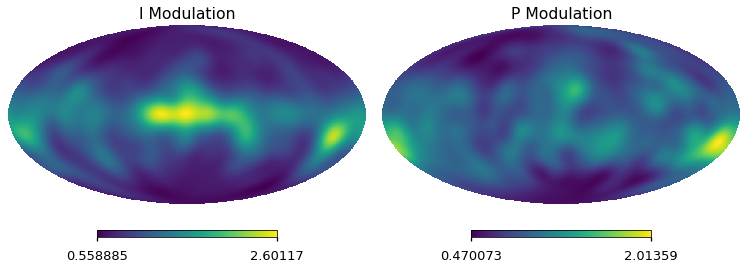
\includegraphics[width=2\columnwidth]{figures/mod_dust.png}\\
     
      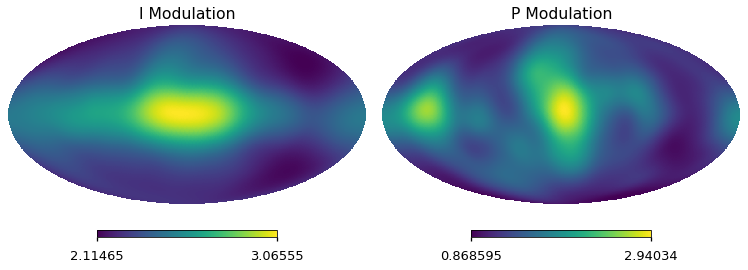
\includegraphics[width=2\columnwidth]{figures/mod_synch.png}\\
     \caption{Modulation maps for (top) dust and  (bottom) synchrotron. }
     \label{fig:modulation_maps }
 \end{figure*}
 

 
We remark here that the synthesis of small scales involves regions far from the Galactic plane.  We adopt the  \texttt{GAL097} \emph{Planck}  mask\footnote{\texttt{HFI\_Mask\_GalPlane-apo2\_2048\_R2.00.fits}} for dust . This is because, inside this area, the dust signal presents a very high SNR that small angular scales (e.g. $\sim20 $ arcmin ) are less affected by noise. We therefore decide to optimally exploit the state-of-art data on dust emission by employing the real small scales from observations nearby the Galactic plane.  

We follow a similar approach also for synchrotron and use the same mask as for dust to include real small scales in the Galactic plane region. Although synchrotron high-resolution data are currently lacking in this region, the inclusion of full resolution data, albeit coarser than the dust ones, surely encodes scales ($\sim 1$ deg) smaller   than   injection scale $\ell_1=38 $.  

To make the transition from the two regions piecewise, we make sure to apodize both masks have been apodized with a Gaussian profile with 5 deg length.



%\subsection{Dust emission}

%\subsubsection{Dust Amplitude}


%We first compute the $tt$, $ee$, and $bb$ power spectra from the dust template $i$, $q$, and $u$ maps and fit each with a power law $A\ell^{\gamma}$ in different multipole ranges depending on the native resolution of the map. Given that the intensity template has been estimated in a different way to the Q and U templates, we employ two different multipole scale cut-offs: $\ell=400$ and $100$, respectively. This further prevents the mixing of scales due to variable resolutions. Specifically, we employ $100 < \ell < 400$ for $tt$ and $30 < \ell < 110$ for $ee$ and $bb$. The spectral indices estimated from the fit are $\gamma = -1.29$, $-0.33$, and $-0.40$ for $tt$, $ee$, and $bb$, respectively.Adopting these values of $\gamma$ directly would lead to the $ee$ and $bb$ power exceeding $tt$ for large enough $\ell$ given the steeper index of the latter. {\bf Some words on why this is ok in principle but gives problems with polarization fraction in practice} We prevent this by adopting a common spectral index $\gamma = -1.29$ to extrapolate all three spectra to higher $\ell$. This choice is further motivated by the fact that the dust intensity template is provided at a higher resolution than the polarization ones, allowing to observe the dust specifics at higher detail with respect to the polarization data being more affected by noise and systematics. Although we are assuming that small scale polarized dust emission to be the same spectral index as the intensity one, this  is something that is physically intuitive and expected   from magneto-hydro dynamic simulations \citep[][]{Kim:2019}. We then generate $iqu$ maps encoding only small scales generated from the fit power law spectra and ranging from the pivot $\ell$-scale up to the multipole related to the desired pixel resolution scale of the dust map we want to simulate.  
%Since we want the small scales to be modulated by the amplitude of the dust emission at large scales, we apply two different modulations for the $i$ and for the $qu$ maps as they are convolved with different beam resolutions. We adopt  the $i$  map   smoothed at 5 deg as a template for both modulation maps.  We then identify a region encoding  low and intermediate Galactic latitudes by masking  all the pixels in the smoothed $i$ map  whose  value is $>4.5 \log ( \mu K )$.  The  intensity modulation is then constructed by performing two different normalization in the regions defined outside and inside  the mask. We use the \emph{MinMax} rescaling ranging   between $1$ and $2$ for the low-intermediate latitudes and between $0.1$ and $1$ for the high latitudes. For the polarization modulation map, we rescale similarly outside the mask between $0.1$ and $1$ but we saturate to   $1$  all the pixels  inside the low latitude region. Once the small scale maps are modulated, they are then co-added to the  low-pass filtered  $iqu$ maps (given the $\ell$-pivot scale) that encode  large scales only. Finally, the $iqu$ maps are transformed   back to the real $IQU$ maps  to perform the validation steps required to assess the quality of the maps. 



\subsubsection{Dust Spectral Parameters}
Smaller angular scales are also included for the dust spectral parameters, by means of extrapolating the power law fitted from the GNILC  maps of $\beta_d$ and $T_d$.  We employ a different procedure with respect to the one presented in Sect. \ref{subsec:methodology}.  
We consider the $I$ map smoothed  at 5 deg.  We then identify two  regions encoding  low and intermediate Galactic latitudes corresponding to the  \texttt{GAL080} \emph{Planck} mask.  The  intensity modulation is then constructed by performing two different normalization in the regions defined outside and inside  this mask.  We \emph{min-max} rescale the map in the area inside the mask so that it  ranges   between $1$ and $2$, whereas    between $0.1$ and $1$ for the high latitudes.

Moreover, we fit the power-law of the $\beta_d$ and $T_d$ power  spectra, in two different multipole ranges, respectively $200-400$ and $100-400$.  Since the fitted power law  indices are  flatter than the one employed for dust amplitudes  $\alpha_{\beta_d}= 0.04$ and $\alpha_{T_d} = -0.47$, we don't expect the  small scales to dominate when rescaling maps at lower and higher frequencies than the reference one ( 353 GHz). 


%\subsection{Synchrotron Emission}
 
\subsubsection{Synchrotron Spectral Parameters}\label{sec:beta_s}
 \textbf{Giuseppe:   } 
 We start from the $\beta_s$ map that has been already employed in the previous suite of PySM models \citet{Thorne:2017}. This map has been produced by combining data from WMAP and HASLAM \citep{mivilledeschenes:2008}. One of the most striking feature of this map is  the lack of information on sub-degree scales. This is an intrinsic limit of radio radio observations as   synchrotron emission  increases  with low frequencies.  However, \citet{Krachmalnicoff:2018} reported a study  on $\beta_s$ estimated from S-PASS data at $2.3 $ GHz and at $10'$ resolution.   Together with a higher level of spatial variations, the authors noted an increase in the variance with respect the one estimated in the $\beta_s$ map derived by \citet{mivilledeschenes:2008}.  In this work, we propose an improved  map of $\beta_s $, starting from the template from \citet{mivilledeschenes:2008} and also benefits of  the recent  S-PASS observations. In particular:  we subtract the offset term from $\beta_s$  and rescale the large scale $\beta_s$   map by a factor $1.572$ as proposed by \citet{Krachmalnicoff:2018}. We than fit a  power-law  in the multipole range  $2<\ell<38$ and estimated $\alpha_{\beta_s}=-0.61 $. We then synthesize  small scales  from the fitted power law,  and modulate them with a modulation map obtained from the intensity HASLAM template. Similarly to what we did for the dust, we  min-max rescaled the modulation map  between 0.1 and 1.1 in the region outside the \texttt{GAL080} mask and from 1.1 to 2 in the region inside. 
 Then we add the modulated small scale  and the  large scale maps, and we make sure also to sum  an offset around $-3.10$.
 
Finally, although small scales of $c_s$  have not been detected yet, we presumably expect as well sub-degree spatial variations for this synchrotron parameter. Small  scales at multipoles $\ell>36$  are therefore  included   assuming them to follow  the same power law as  the $\beta_s$ ones,  i.e. $\alpha _{c_s}=\alpha _{\beta_s} = -0.61$, and that are  modulated with the exact same modulation map as the one we  adopted for $\beta_s$.

\section{Layer Model} \label{sec:layers}
%writing: jacques

Evidence for variation of Galactic foreground emission laws as a function of frequency across the sky also implies that emission laws must vary along the line of sight. As a consequence, we anticipate that dust emission, if locally matching a modified blackbody in the form of equation \ref{eq:dust-emission-law}, is seen by an observer as a superposition (an integral along the line of sight) of modified blackbodies -- which is not a modified blackbody. In addition, if along the line of sight different line elements emit polarized radiation with different polarization angles, the frequency scaling should vary between $I$, $Q$ and $U$. To model this complexity, a multilayer dust emission model based on an implementation of the approach of \cite{Martinez-Solaeche:2018} in the PSM software (version 2.3.3) has been implemented in PysM 3.

The PSM has been run to produce six maps of dust emission at 353~GHz (intensity and polarization, for a total of 18 Healpix maps at {\tt nside=2048}), and six maps of dust spectral index $\beta_d$ and dust temperature $T_d$, also at {\tt nside=2048}, following the approach described in \cite{Martinez-Solaeche:2018}. The PySM software uses these maps as inputs, and generates the dust Stokes parameters maps as:
\begin{equation}
    S_\nu(p) = \sum_{i=1}^6 S^i_{\nu_{\rm ref}}(p)
    \left( \frac{\nu}{\nu_{\rm ref}} \right)^{\beta^i_d(p)}
    \frac{B_\nu(T^i_d(p))}{B_{\nu_{\rm ref}}(T^i_d(p))},
\end{equation}
where $S_\nu(p)$ stands for any of the three Stokes parameters of interest, $I$, $Q$ and $U$, at frequency $\nu$ and in pixel $p$, and superscripts $i$ indicate the layer, from 1 to 6.

In the implementation used here, the 353~GHz templates for the six emission layers are slightly different from those of \cite{Martinez-Solaeche:2018} as we employ more recent Planck data products. Large scale polarized emission maps are the GNILC maps obtained in \cite{planck2016-l04} using the method developed by \cite{2011MNRAS.418..467R}. These are complemented by small scale realizations with scale dependence matching the $I$, $E$ and $B$ dust spectra measured in \cite{planck2016-l11A}, modulated by the large scale local intensity and polarized intensity level. This process filters some of the real small scale power in dust intensity and polarization maps, replacing it with random fluctuations, and thus does not quite reproduce the non-Gaussian and non-stationary properties of real dust emission. Improving the generation of small scale fluctuations is left to future work.

% \item Methodology, especially the connection between MKD and what we implement in PySM. What capabilities of PySM can we exploit to extend MKD?
%  \item Comments on any numerical trickiness, e.g., p > 1

\section{Map Validation} \label{sec:validation}
\begin{enumerate}
    \item Define suite of tests
    \item Compare models in interesting spaces, e.g., decorrelation, EE/BB
    \item Zoom in on B/K patch, other regions
    \item Non-gaussianity of polarization fraction tensor formalism
    \item Susan's student's plot of maps x galaxy catalogs (a la Chiang and Menard) to demonstrate CIB mitigation
\end{enumerate}

\textbf{Ben:} In this section we validate the foreground model developed in Section~\ref{sec:small_scales}. \sg{In Section~\ref{sec:sync_validation} we compare the power spectra of different synchrotron models with BeyondPlanck synchrotron map for temperature, and LFI 30 GHz for polarization. We find a reasonable agreement between the data and our models for different fraction of the galactic synchrotron signal masked.} In Section~\ref{sec:dust_validation} we will demonstrate that the two-point statistics of the stochastic small scales are properly modulated for different regions of sky defined by Galactic masks of varying size. We will also assess the properties of our dust model in the small patch of sky observed by the BICEP / Keck telescopes and the South Pole Telescope. In Section~\ref{sec:nongaussianity}, we will assess the level of non-Gaussianity introduced by the log polarization tensor formalism, and compare this to the case of a purely Gaussian small scale model which has been modulated by a Galactic template. 

\subsection{Synchrotron validation} \label{sec:sync_validation}
\textbf{Shamik:} In this section we detail the validation of the new synchrotron models by comparing them with BeyondPlanck synchrotron map for temperature, and LFI 30 GHz observations for polarization. We compare the model with data at map level and by computing the power spectra. For validating the PySM synchrotron temperature models, we use the synchrotron map from the BeyondPlanck re-analysis of Planck LFI data \citep{2022arXiv220108188A}. The BeyondPlanck release 1 synchrotron map is at a reference frequency of 30\,GHz at $2^\circ$ angular resolution. We produce single frequency temperature maps for the different synchrotron models at 30\,GHz and smoothed with a Gaussian beam with FWHM = $2^\circ$.

In case of the synchrotron polarization, we are comparing the models with band integrated observations. So, we compute bandpass integrated maps of the different synchrotron models. For this purpose we use the average LFI 30\,GHz RIMO transmission \citep{planck2014-a03}. The bandpass integrated maps are further smoothed with Gaussian beams of 33.1 arcmin beams to produce model maps at native resolutions of the LFI 30 GHz data. The observed power spectra are computed by taking a cross spectra between A and B splits of the NPIPE (PR4) 30 GHz maps \citep{planck2020-LVII}.

%\subsubsection{Galactic masks}
The polarized synchrotron power spectra validation is performed on the full sky and with sky masks with 70\% and 50\% sky fractions. To produce the 70\% and 50\% masks we use the LFI 30\,GHz map of polarized intensity, smoothed with a Gaussian beam of $2^\circ$ FWHM, and masking pixels above 17 and 10 $\mu{\rm K}_{\rm CMB}$, respectively. These masks are shown in Figure \ref{fig:sync_masks}. We apodized these masks with a $2^\circ$ cosine apodization.
\begin{figure}
    \centering
    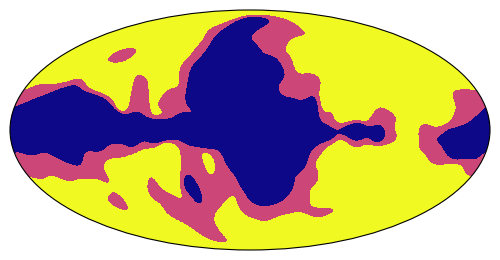
\includegraphics[width=0.46\textwidth]{figures/sync_galactic_mask.png}
    \caption{Figure showing the two different Galactic masks used for the synchrotron validation. The yellow region is included by the 50\% sky mask, while the 70\% mask additionally includes the pink region.}
    \label{fig:sync_masks}
\end{figure}

We use HEALPix \footnote{https://healpix.sourceforge.io} \texttt{anafast} function \citep{2005ApJ...622..759G, 2019JOSS....4.1298Z}  to compute the power spectra for the model and observation maps. For the polarization analysis, both the model and the LFI maps are additionally masked with an apodized polarized point source mask. We do not use a pseudo-$C_\ell$ estimator as the synchrotron signal is not statistically isotropic, and we correct for the partial sky by naively dividing by an $f_{\rm sky}$ factor.

\begin{figure}
    \centering
    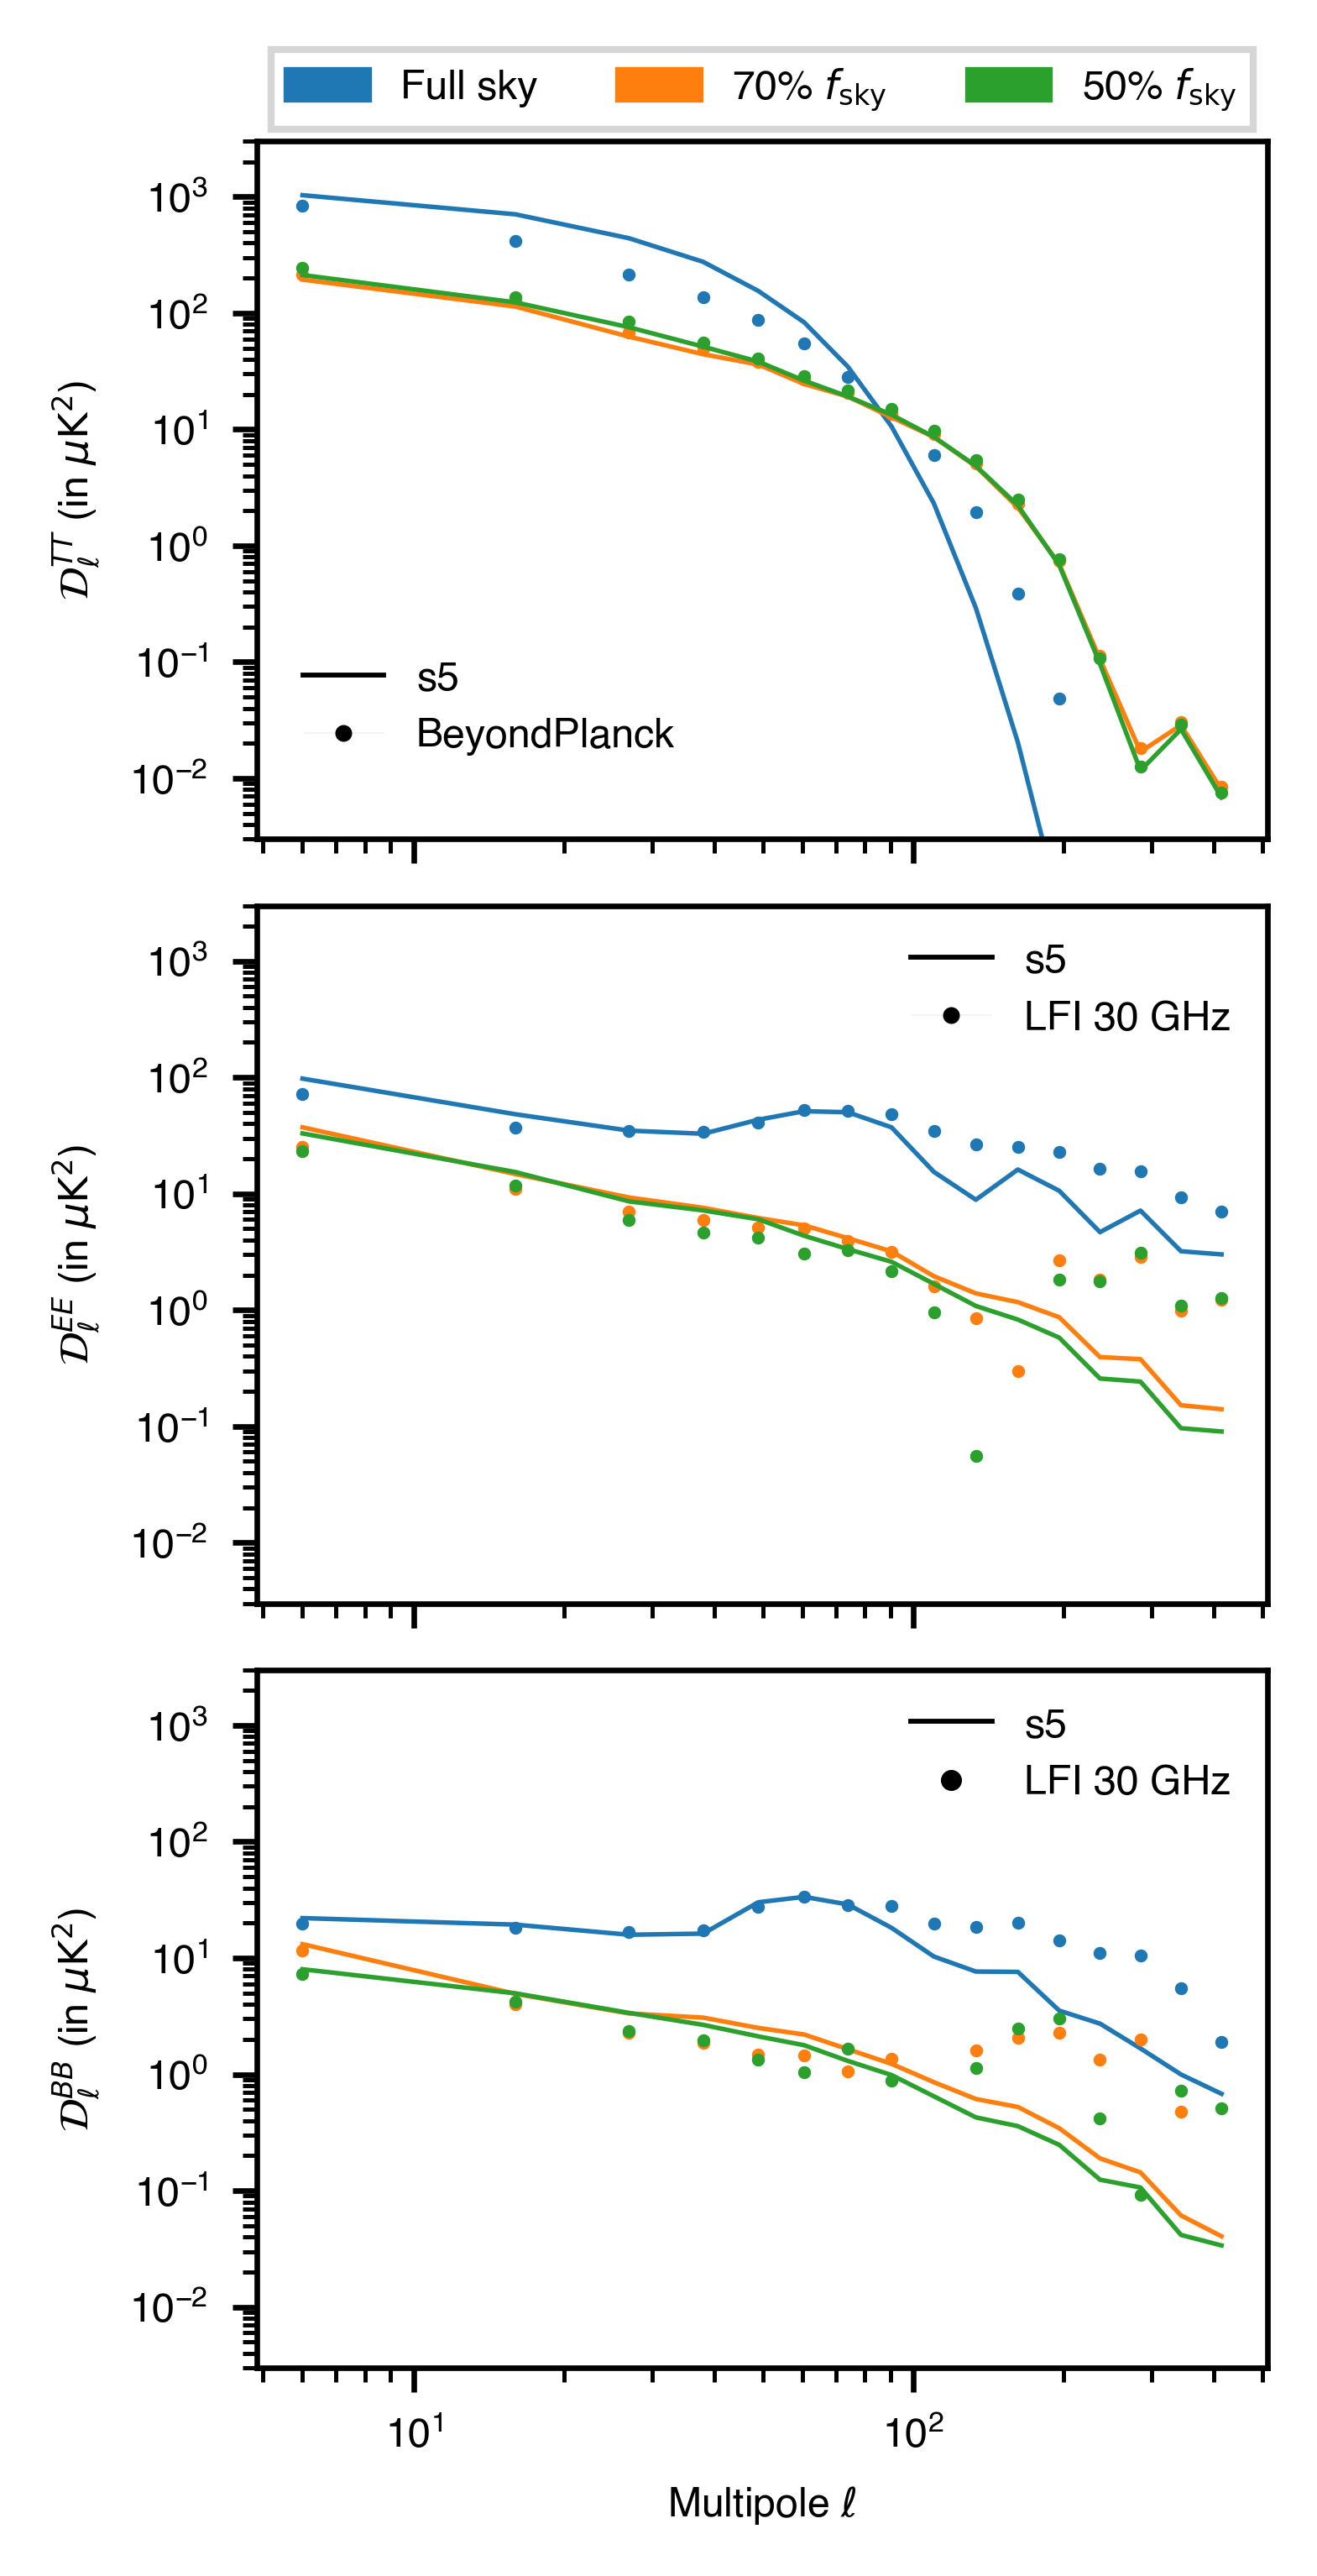
\includegraphics[width=0.48\textwidth]{figures/Dlcomp_PySM3-4b7_s5_vs_BPnLFI30_BPI.png}
    \caption{Figure showing comparison of power spectra of the PySM s5 model with observation on different sky fractions. The spectra obtained for models s4, s6 and s7 are similar so we don't show them here. The $TT$ power spectrum comparison is done with synchrotron maps from BeyondPlanck release 1. The $EE$ and $BB$ power spectra is compared with NPIPE LFI 30\,GHz map. The LFI 30\,GHz spectra are computed as a cross spectra between the NPIPE splits A and B.}
    \label{fig:Dl_sync_galmask}
\end{figure}

The $TT$, $EE$ and $BB$ power spectra comparisons, for model s5, are shown in Figure~\ref{fig:Dl_sync_galmask}. The comparison for models s4, s6 and s7 have nearly identical results. The $TT$ power spectra for masked skies show excellent agreement with the BeyondPlanck synchrotron temperature power spectra. However, there is poor agreement for the full sky power spectra. On the full sky most of the spectra is dominated by what happens in the Galactic plane, which for observational data is contaminated by free-free and anomalous microwave emission (AME). Despite the BeyondPlanck component separation, the synchrotron power in the brightest sky regions are likely to have some residual contamination and associated uncertainty. So, it is reasonable to argue that for synchrotron temperature there is excellent agreement for all but the brightest parts of the sky, where the comparison is harder to make at 30\,GHz. For polarization we find reasonable agreement at $\ell \lesssim 100$. For $\ell > 100$ the PySM synchrotron models typically have less power than the data. However, an important caveat is that despite the point source masking, there is some residual radio point source contribution to this power in the LFI maps.

\begin{figure}
    \centering
    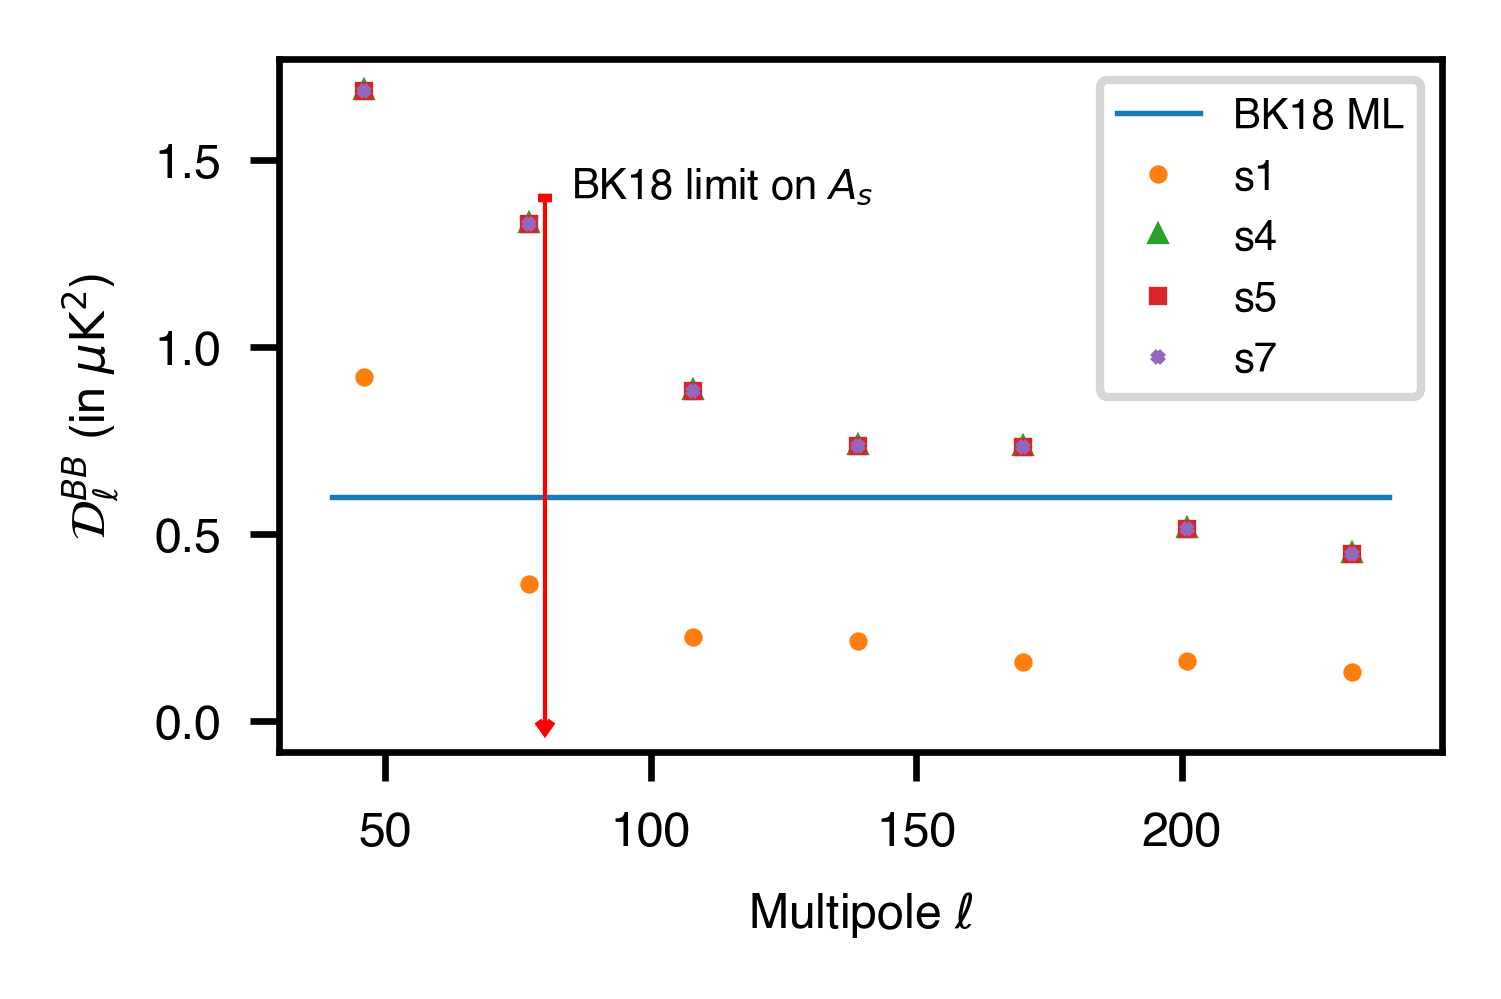
\includegraphics[width=0.49\textwidth]{figures/Dlcomp_PySM3-4b8_BKpatch.png}
    \caption{Figure showing comparison of power spectra in the BICEP/Keck patch for the new PySM synchrotron models s4, s5 and s7 with old synchrotron model s1 and the limits on the synchrotron power obtained in BICEP/Keck 2018 \citep{Ade:2021} at the reference frequency of 23 GHz. The blue line shows the BICEP/Keck 2018 maximum likelihood model for synchrotron with $A_s=0.6 \mu {\rm K}^2$, $\alpha_s=0$. The red arrow indicates the BICEP/Keck 95\% confidence upper limit on $A_s<1.4 \mu {\rm K}^2$ after marginalizing over $-1<\alpha_s<0$ at $\ell=80$. Note that the PySM synchrotron model s4, s5 and s7 have identical spectra.}
    \label{fig:Dl_sync_BK}
\end{figure}

\subsubsection{BICEP / Keck patch}
The cleanest patch of sky in the southern hemisphere is particularly important for ongoing and future CMB experiments that target measurement of the primordial CMB B-modes. We focus on the small clean patch of sky that is targeted for the BICEP/Keck experiment for their constraints on the tensor-to-scalar ratio. This overlaps with the tentative sky patch that will be targeted by the CMB-S4 experiment for their primordial B-mode search. In their 2021 analysis the BICEP/Keck team placed a upper limit of $A_s<1.4 \mu{\rm K}^2$ at a pivot frequency of 23\,GHz with $\beta_s=-3.1$ after marginalizing over the range $-1<\alpha_s<0$ \citep{Ade:2021}. The BICEP/Keck maximum likelihood model for the synchrotron spectra is parameterized by $A_s=0.6 \mu{\rm K}^2$, $\beta_s=-3.0$ and $\alpha_s=0$. In Figure~\ref{fig:Dl_sync_BK}, we compare these two sets of constraints from the BICEP/Keck 2018 results with the new PySM synchrotron models s4, s5 and s7. We also plot the old PySM s1 synchrotron model to show how the synchrotron model has changed in this patch of interest.

The new synchrotron models, s4, s5 and s7, have more power in the BICEP/Keck patch when compared to the old s1 synchrotron model. The latest BICEP/Keck results only has weak detection of synchrotron. We find that both the old and new PySM models are consistent with the BICEP/Keck upper limit on the synchrotron power. However, the BICEP/Keck maximum likelihood model for synchrotron has a better agreement with the new synchrotron models s4, s5 and s7 than with the old s1 synchrotron model. Thus, the new small scale generation in the synchrotron models s4, s5, and s7 increases the synchrotron power in the BICEP/Keck patch and is in better agreement with the constraints from the latest BICEP/Keck results.

\subsection{Dust validation} \label{sec:dust_validation}

\textbf{Ben:} In this section we calculate the power spectra of the dust template described in Section~\ref{sec:small_scales} using a variety of Galactic masks derived for the analysis of Planck data. We also present power spectra calculated on the region of sky observed by the BICEP Array and SPT-3G experiments. This latter case will assess how the small scale model performs in small areas of high latitude sky, which are vital for future constraints on the tensor-to-scalar ratio. Primarily, we will demonstrate that the spatial modulation of the small-scale realizations does not add too much foreground power in areas of high latitude sky, which has been a criticism of previous PySM models. 

All power spectra in this section are computed using the {\tt NaMaster} code \citep{Alonso:2019}. 

\subsubsection{Planck Galactic masks} \label{sec:galactic_spectra}

\textbf{Ben:} In this section we present power spectra computed on Galactic masks of varying sizes. We define a set of Galactic masks starting from the unapodized Galactic masks\footnote{\texttt{HFI\_Mask\_GalPlane-apo0\_2048\_R2.00.fits} distributed \url{https://pla.esac.esa.int}} by the Planck collaboration via the Planck Legacy Archive. There are eight masks in total, leaving between 20\% and 99\% of the sky available for analysis. We apodize each mask with a cosine taper of characteristic length $2^\circ$ resulting in nine masks: \texttt{GAL015}, \texttt{GAL034}, \texttt{GAL052}, \texttt{GAL062}, \texttt{GAL072}, \texttt{GAL082}, \texttt{GAL092}, \texttt{GAL096}, where the number indicates the percentage of the sky left for analysis, i.e., $100 f_{\rm sky}$.  

In Figure~\ref{fig:spectra_by_field} we show the $TT$, $EE$, and $BB$ power spectra of the \dnine{} model, and of the GNILC maps from which the \dnine{} model was derived, computed on four of the Galactic masks described above.

\begin{figure}
    \centering
    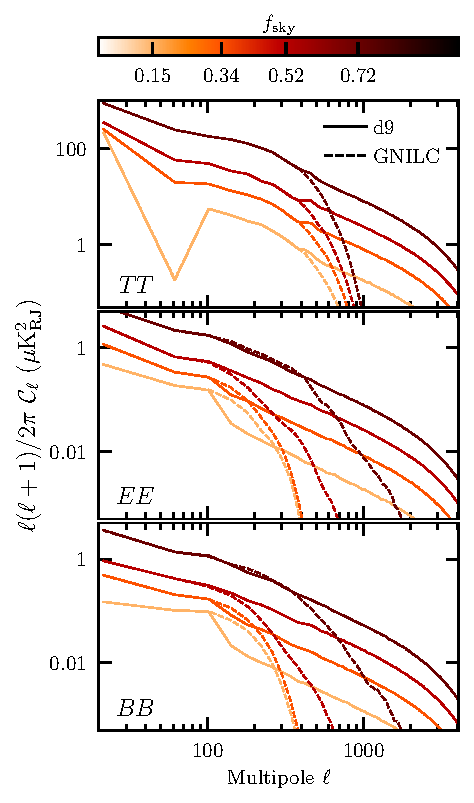
\includegraphics{paper_spectra_by_field_NSIDE2048.pdf}
    \caption{This figure compares the power spectra of the \dnine{} model (solid lines) and the input GNILC map (dashed lines) when computed on the \texttt{GAL015}, \texttt{GAL034}, \texttt{GAL052}, and \texttt{GAL072} Galactic masks.}
    \label{fig:spectra_by_field}
\end{figure}

\subsubsection{Small Field Power Analysis} 
%Kenny's analysis here

\textbf{Kenny:} To compare the small-scale performances of the latest PySM dust models \texttt{d9}, \texttt{d10} and \texttt{d12} with real data, we mainly follow the analysis method described in \cite{planck2014-XXX} to examine the model behaviors. We first use a HEALPix grid with $\texttt{nside} = 8$ to divide the full sky into 768 patches. At the center of each patch, we create a 400-square-degree circular mask with its edge tapered by a $2^\circ$ FWHM Gaussian (resulting in $f_{\rm sky} \approx 0.008$), and apply such a mask to the mean-subtracted dust model and NPIPE half-ring split maps at 353~GHz. We then use \texttt{anafast} to compute the binned $BB$ auto-spectra of the masked model maps at $\ell = 55,90,135,190,255,330$ with $\Delta \ell = 30$, and scale them to be the full-sky $\mathcal{D}_\ell^{BB}$ by dividing the apodization mask integral squared. For the masked NPIPE data maps, we instead compute cross-spectrum from the two split maps to minimize the noise correlation. The representative results from two selected circular fields at $|b| > 35^\circ$ of the northern and southern Galactic hemispheres are shown in Fig.~\ref{fig:smallfield_power}. (\textbf{Kenny:} this analysis uses anafast - contradicts with the NaMaster stated above?)

\begin{figure}
    \centering
    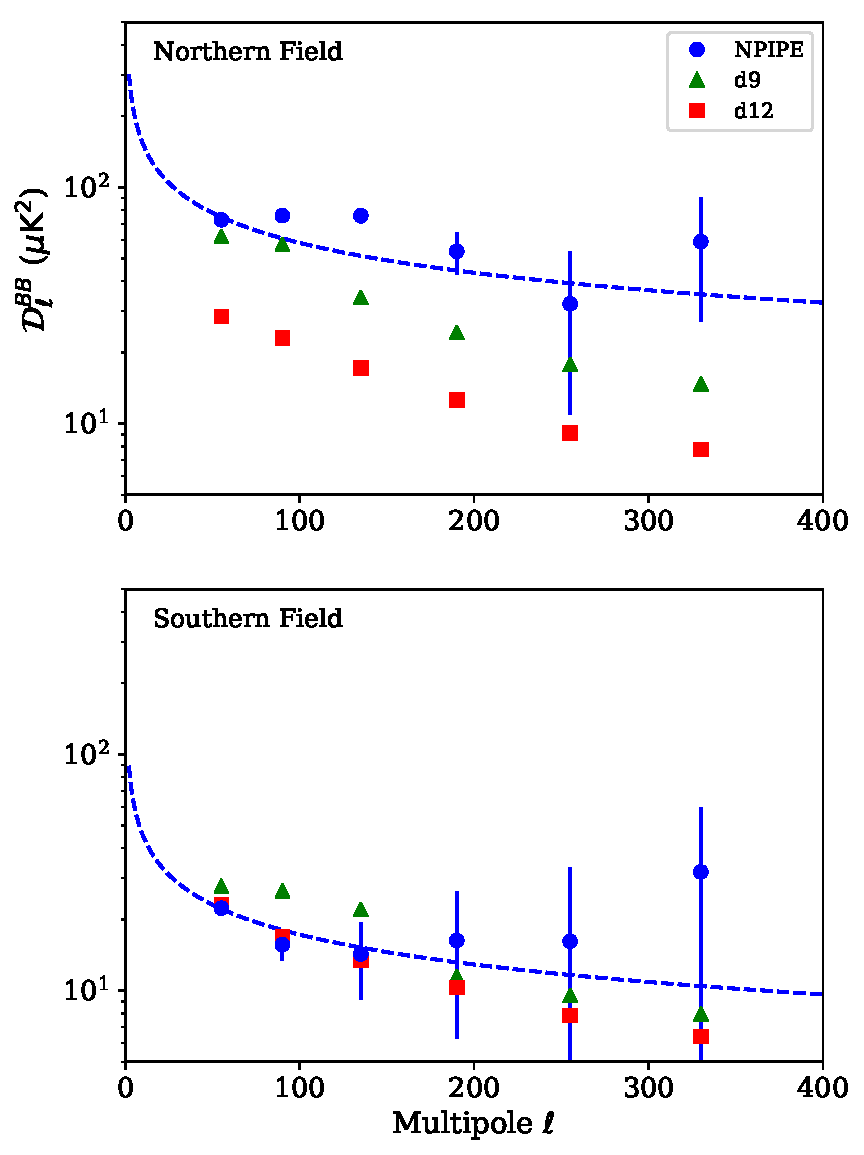
\includegraphics[width=0.48\textwidth]{figures/smallfield_power.pdf}
    \caption{The binned $BB$ power spectra from the 353~GHz NPIPE half-ring split maps and dust model maps \texttt{d9} and \texttt{d12}. The model maps are integrated with a 353~GHz delta bandpass and the NPIPE data maps are color-corrected (i.e., scaled by a factor of 0.92) to the same single frequency. The dashed lines indicate the best-fit of the fixed-index power law on the NPIPE maps, which is largely driven by the first two band powers. Note that we only show the \texttt{d9} results as this model is identical to \texttt{d10} at 353~GHz.}
    \label{fig:smallfield_power}
\end{figure}

We in addition run a fixed-index fit $\mathcal{D}_\ell^{BB} = A^{BB} \big( l/80 \big)^{\alpha^{BB}+2}$ where $\alpha^{BB} = -2.42$ to the $BB$ power spectra. We find that the NPIPE map spectra agree with such a power law within their noise level in nearly all small fields. The \texttt{d9} and \texttt{d10} dust models can basically reproduce the same amplitude $A^{BB}$ in their own fits, while \texttt{d12} produces an amplitude which is somewhat smaller. These models also demonstrate some successes in following the power law up to $\ell \approx 350$, although their agreements are not as close as those of the data. If we define the ratio of the first two band powers to the last four band powers as a proxy for describing the spatial power change across the modulation scale, while the perfect fixed-index power law yields a value of $\approx 1.60$, the NPIPE maps give $1.65 \pm 0.68$ and the \texttt{d9}/\texttt{d10} (\texttt{d12}) model map gives $2.37 \pm 0.77$ ($2.24 \pm 0.87$) over sky patches with $|b| > 30^\circ$.

\subsubsection{BICEP / Keck} \label{sec:bkspt_spectra}

\textbf{Ben:} The current upper limit on the tensor-to-scalar ratio is set by a combination of BICEP / Keck (BK), Planck, and WMAP data: $r < 0.036~(95\%)$ \citep{Ade:2021}. Over the next few years, a collaborative effort between the South Pole Telescope (SPT) and BICEP / Keck will combine high-resolution SPT-3G observations with BK observations in order to ``delens'' the observed CMB B-modes, and further constrain $r$. Therefore, there will be continued interest in simulating Galactic foregrounds on this particular patch of sky.

In Figure~\ref{fig:d1d9_bkpatch} we compare the BB power spectrum of the new \dnine{} model with the original PySM \done{} model, the GNILC input map, and the maximum likelihood dust model in this patch of sky determined from a combination of BK, Planck and WMAP data \citep{Ade:2021}. Model \done{} clearly has excess dust BB power compared to the measured amplitude in this patch of sky, which has been known for some time. This is somewhat ameliorated in model \dnine{}, primarily due to the steeper spectral tilt of the \dnine{} model leading to a factor of $\sim 10$ decrease in power relative to \done{} by multipoles of $\ell \gtrsim 300$. At larger scales of $\ell \lesssim 50$ both the \done{} and \dnine{} models are dominated by the underlying GNILC template, rather than the simulated small scale realizations, and so the mismatch in amplitude between the BK maximum likelihood model and our templates is most likely due to residual noise in the GNILC template. Indeed, most of the constraining power on dust BB power in Ref~\cite{Ade:2021} is driven by BK observations at 220\,GHz, which are not used to inform our model. 

One may argue that the amplitude and spectral tilt of the \dnine{} model clearly disagree with existing observations in the BK patch of sky. While this is true, it is beyond the scope of this work to provide full sky simulations that guarantee consistency with all sets of full sky and partial sky observations. Indeed, the use of power spectrum-based techniques requires a certain amount of global averaging of power spectrum parameters that are in fact known to vary across the sky \cite{planck2016-l04}. For example, while the dust amplitude can be modulated by the use of a large scale template, the spectral tilt has to be fixed to a single value for the full sky, which is not realistic. 

\begin{figure}[ht]
    \centering
    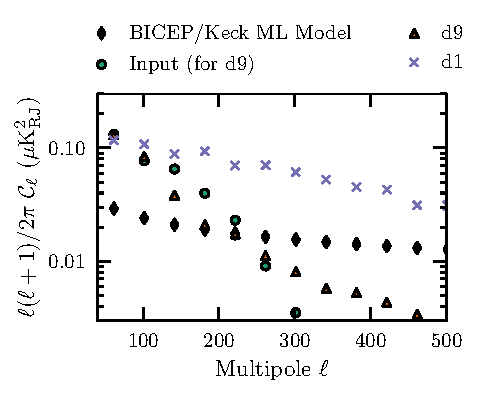
\includegraphics{paper_BK_patch.pdf}
    \caption{This figure shows the BB power spectra of the \done{} (crosses), \dnine{} (triangles), and varres GNILC map (circles), compared to the maximum likelihood BK dust model (black diamonds) derived from a combination of WMAP and Planck with BICEP / Keck data up to the 2018 observing season. Note that in order to make a meaningful comparison between the bandpowers calculated from maps and the theory curve, we first convolve the theory spectrum with the mode-coupling matrix and then compute the decoupled bandpowers by applying the inverted binned coupling matrix.}
    \label{fig:d1d9_bkpatch}
\end{figure}

\subsubsection{Map level validation}
%In this section, we present a map-level validation of the PySM dust models \dnine{}, {\tt d11}, {\tt d12} models against the Planck third data release (PR3) \cite{}.
\textbf{Elisa}: In this section, we compare at the map level, Planck third data release PR3 \cite{planck2016-l03}) and PySM dust models \dnine{}, {\tt d11}, {\tt d12} models. We study how well the modeled intensity $I$ and polarized intensity $P = \sqrt{U^2 + Q^2}$ match the observations on three selected $16.7^\circ \times 16.7^\circ$ patches of the sky, at different frequencies of 217~GHz, 353~GHz and 857~GHz. Here, we focus on two local patches: close to the Galactic plane ($[l,b] =[180^\circ,-10^\circ]$) and, centered on the Bicep / Keck field ($[l,b] =[318^\circ,-61^\circ]$).
Similar to Section~\ref{sec:sync_validation}, we integrate the dust models within the Planck passbands to enable direct comparison. For comparison of intensity maps, we subtract a Wiener-filtered CMB temperature anisotropies map from SMICA and adjust the zero level of the PR3 data to that of the simulated map over regions of faint dust intensity on the sky.
The mask used to adjust the zero levels is shown in figure \ref{fig:mask_zero_lvl_int}. These corrections are not required for comparing polarization data.
\begin{figure}[ht!]
    \centering
    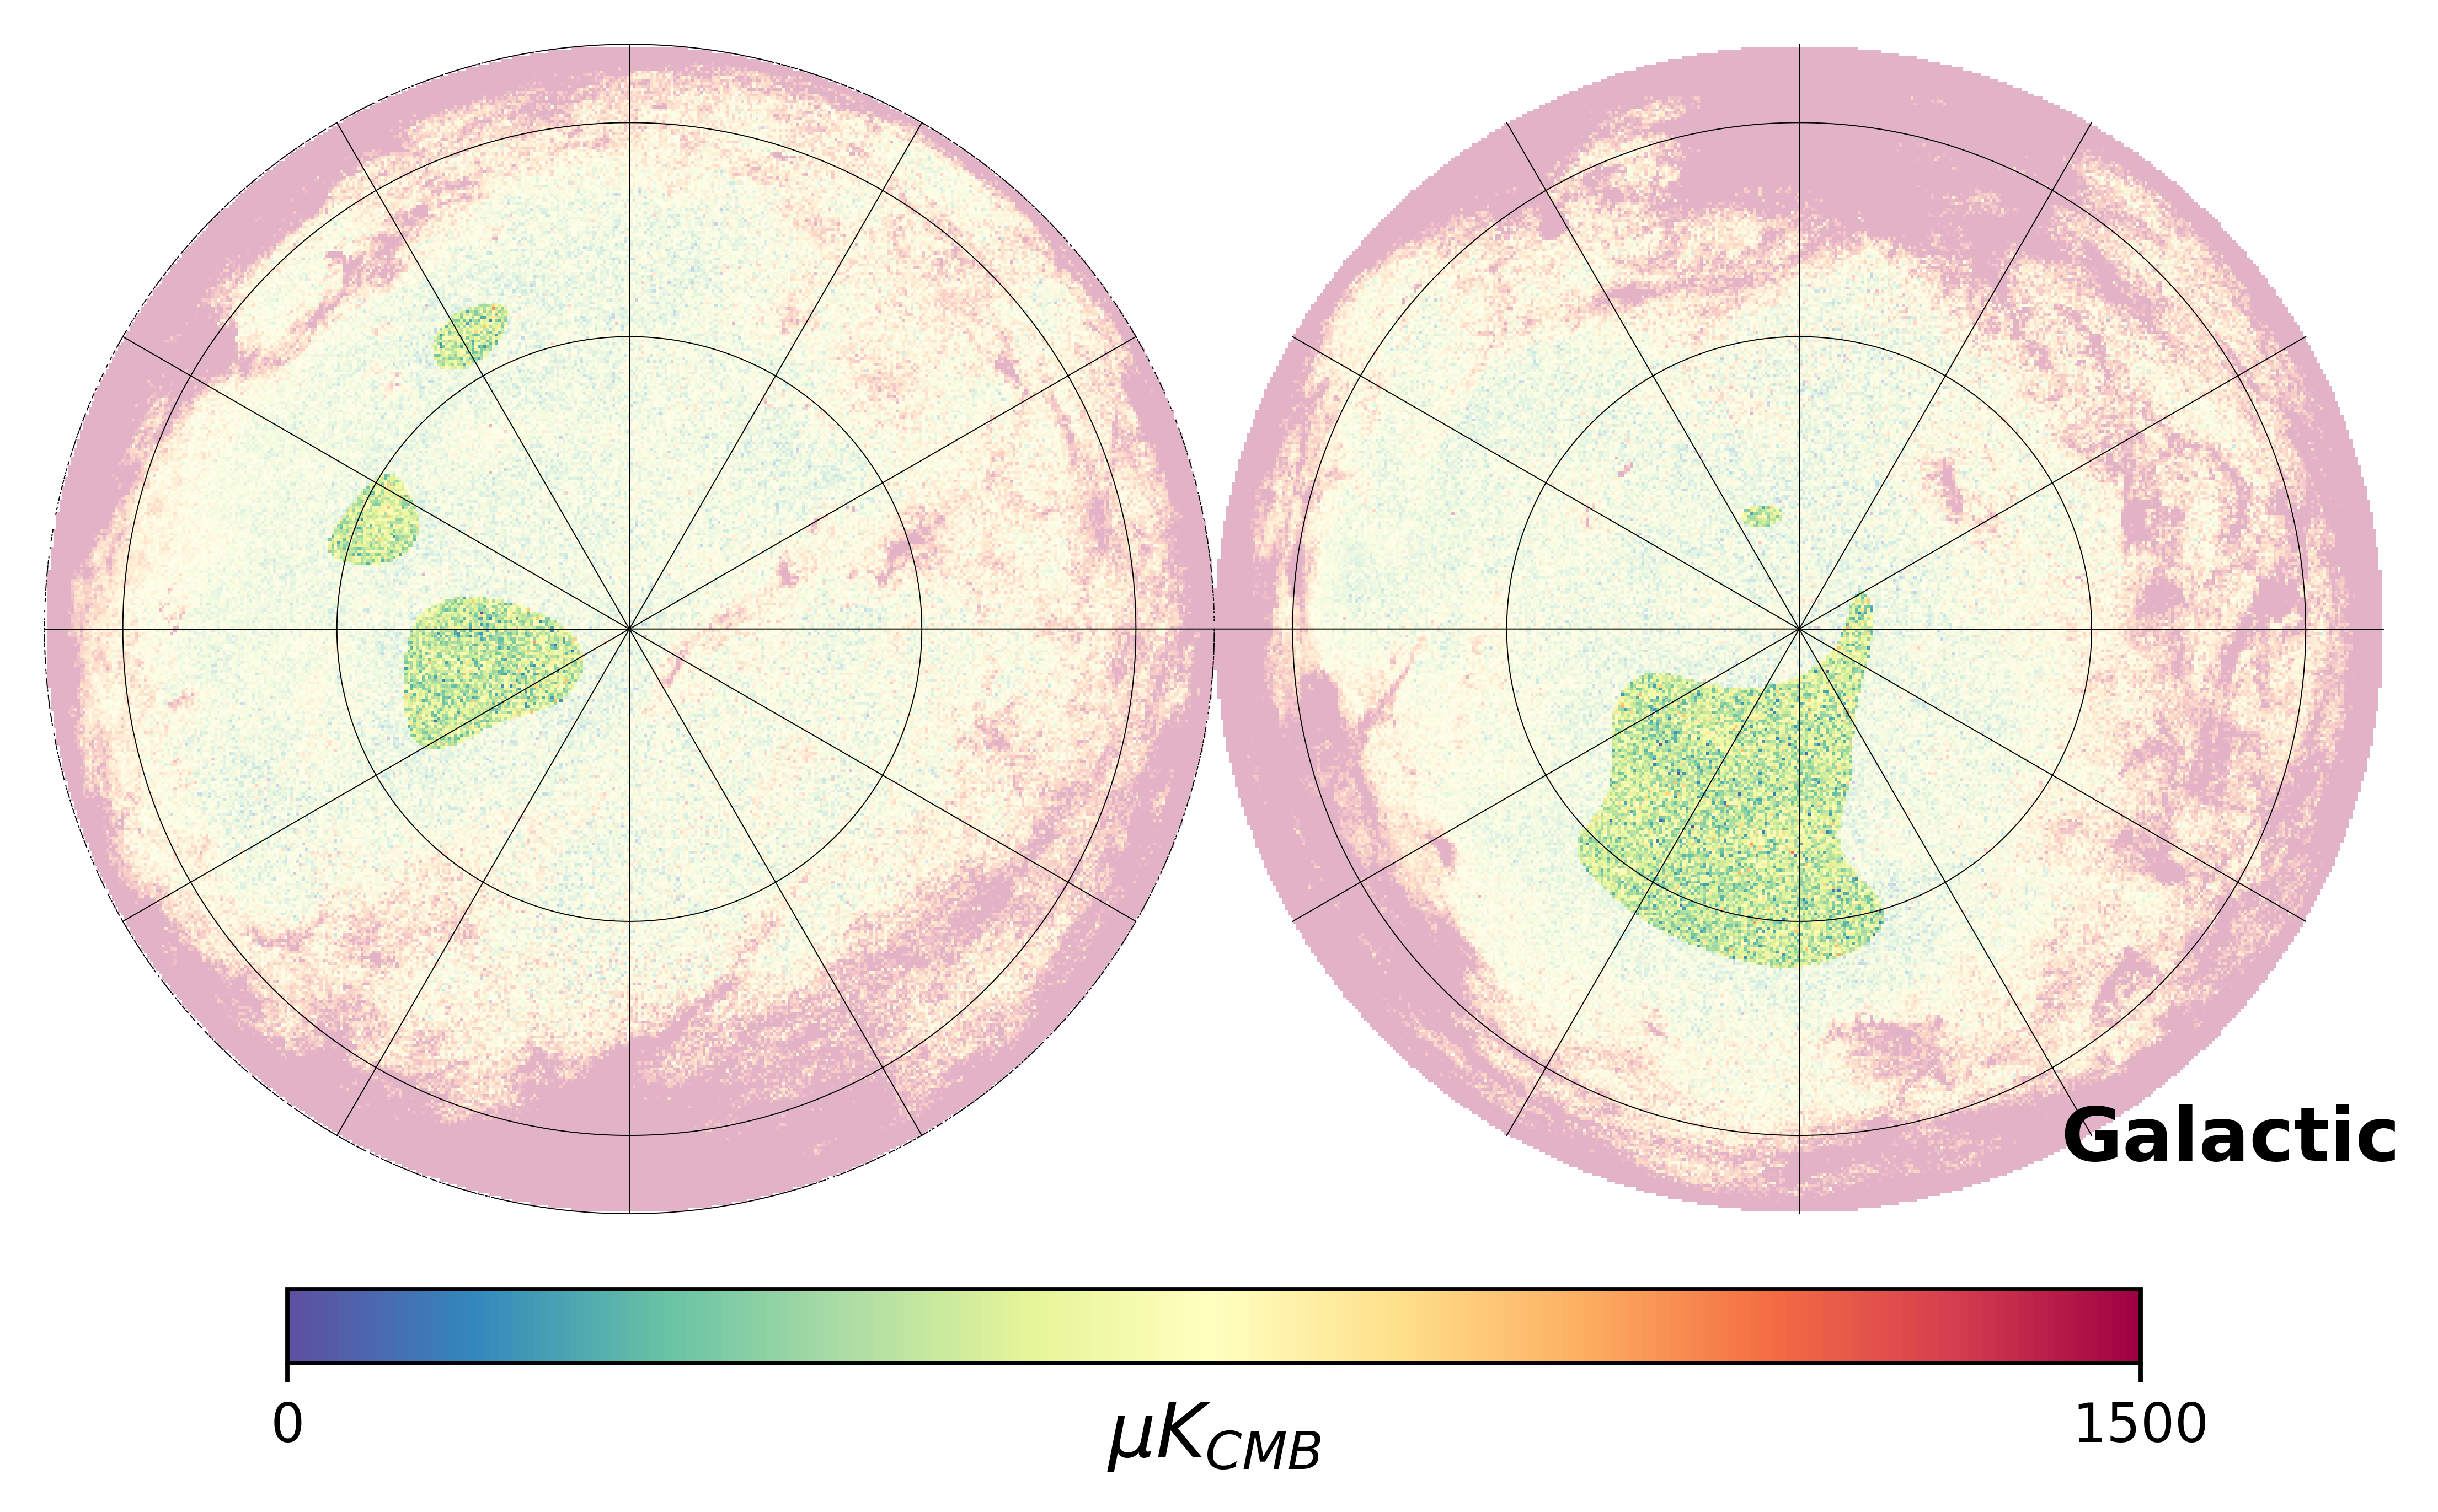
\includegraphics[width=0.48\textwidth]{figures/mask_intxPR3_zero_lvl.png}
    \caption{Mask $\times$ PR3 intensity used to estimate the zero level of PR3 intensity. This mask is obtained by thresholding the intensity of the smoothed PR3 intensity to preserve only the regions where the dust is very low, to estimate the zero-level of the data and models.}%more details
    \label{fig:mask_zero_lvl_int}
\end{figure}

\begin{figure}[ht!]
    \centering
    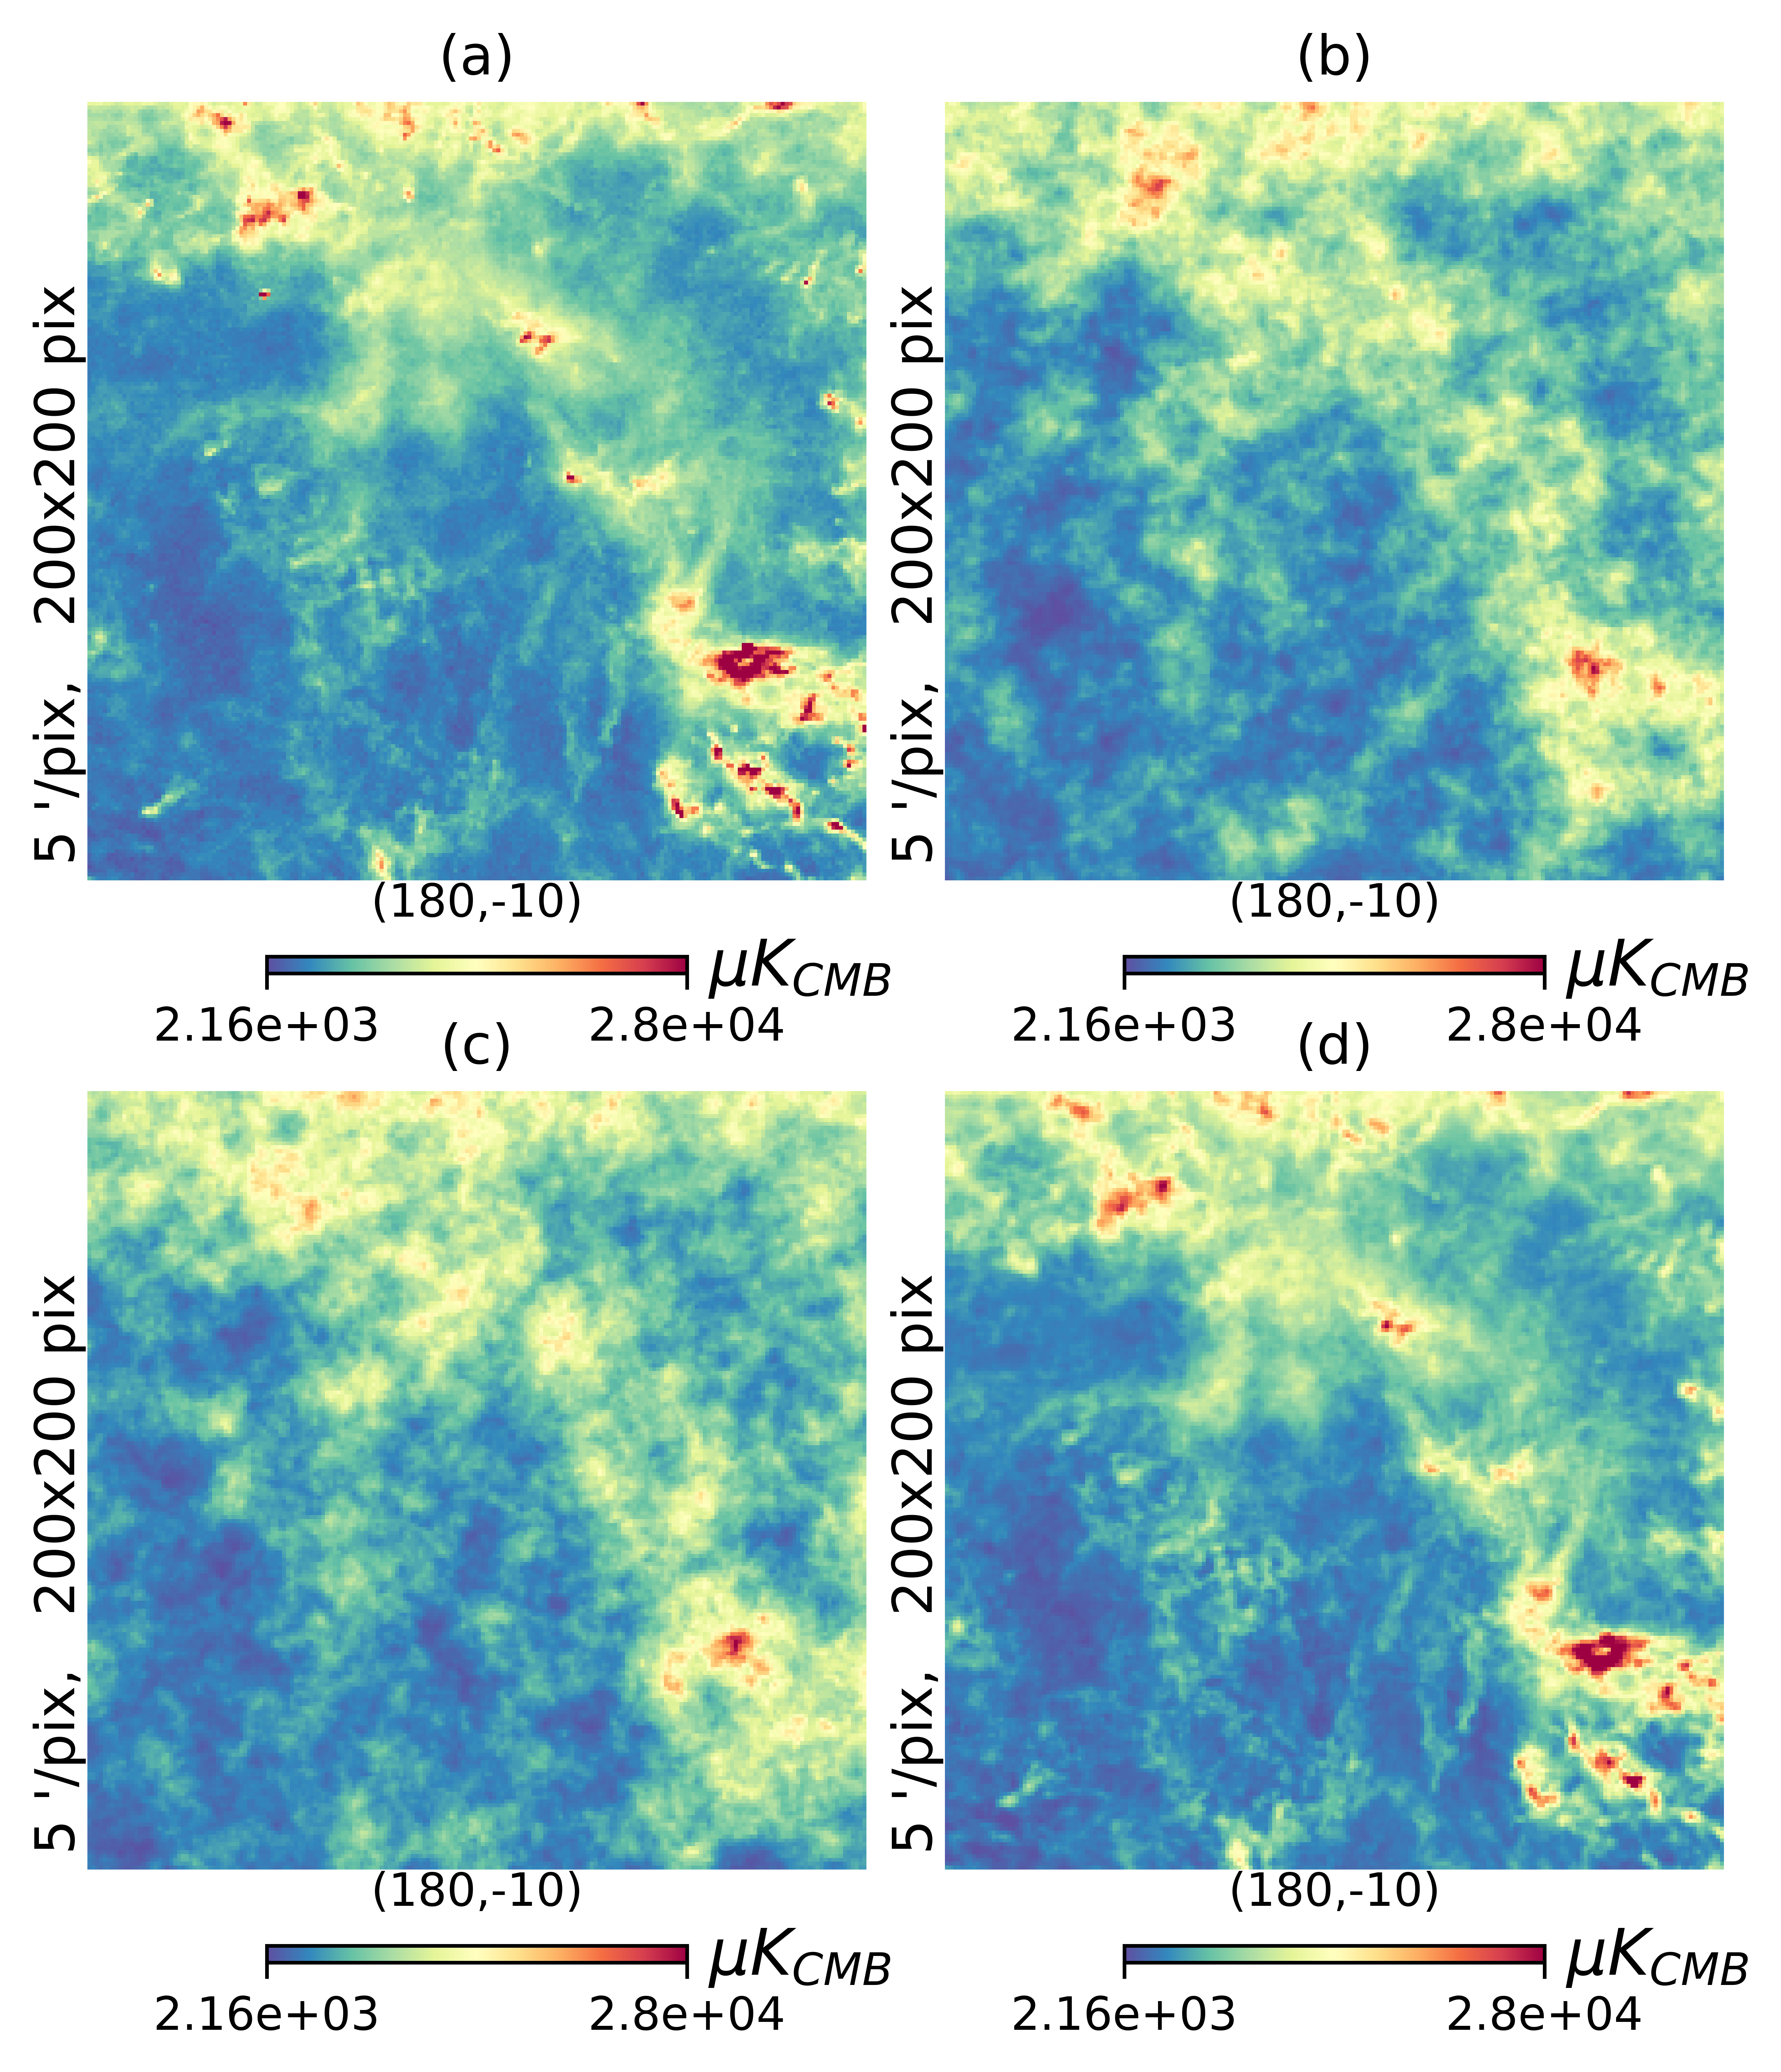
\includegraphics[width=0.48\textwidth]{figures/gal_plane_non_smooth_wo_zero_lvl.png}
\caption{Dust intensity at 353GHz at [l = 180, b = -10] with an angular resolution of 4.41': (a) PR3 (b) d9 (c) d11 (d) d12}    
\label{fig:353_int_gal_plane}
\end{figure}
% \begin{figure}
%     \centering
%     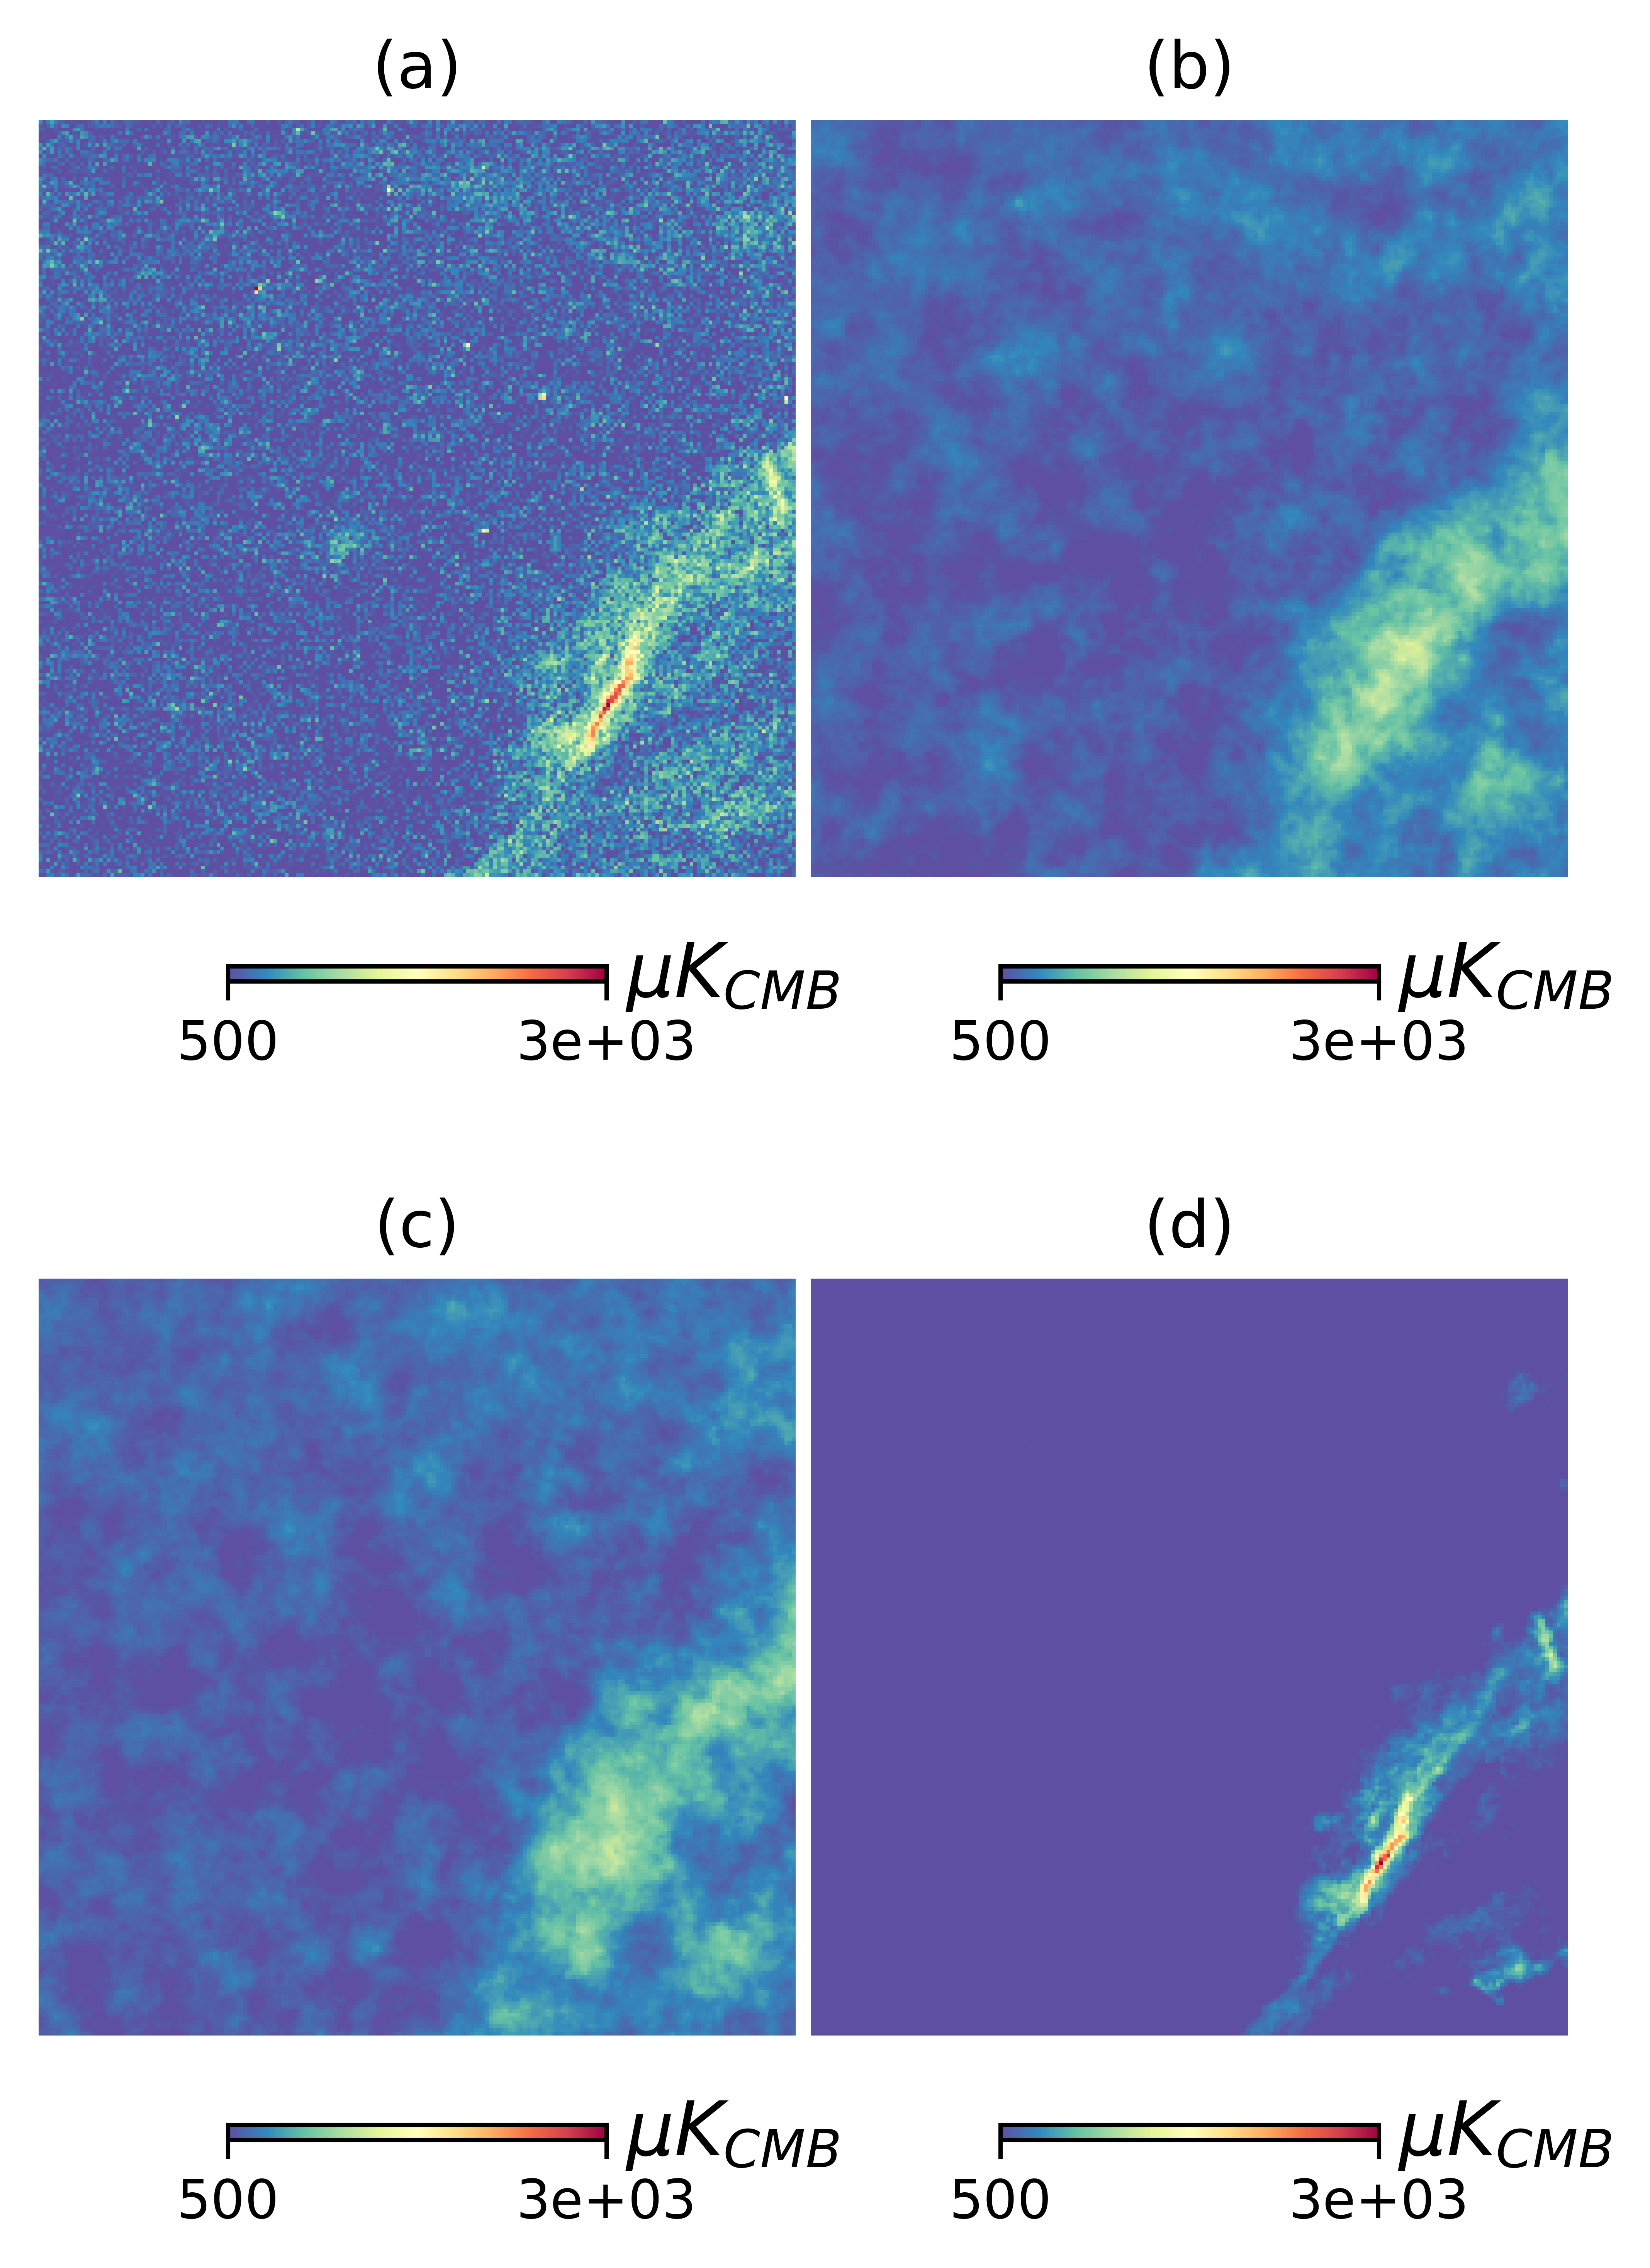
\includegraphics[scale = 0.6]{figures/NGP_non_smooth_wo_zero_lvl.png}
%     \caption{Dust intensity at 353GHz centered at [l = 0, b = 90]: (a) PR3 (b) d9 (c) d11 (d) d12}
%     \label{fig:353_int_NP}
% \end{figure}
\begin{figure}[ht!]
    \centering
    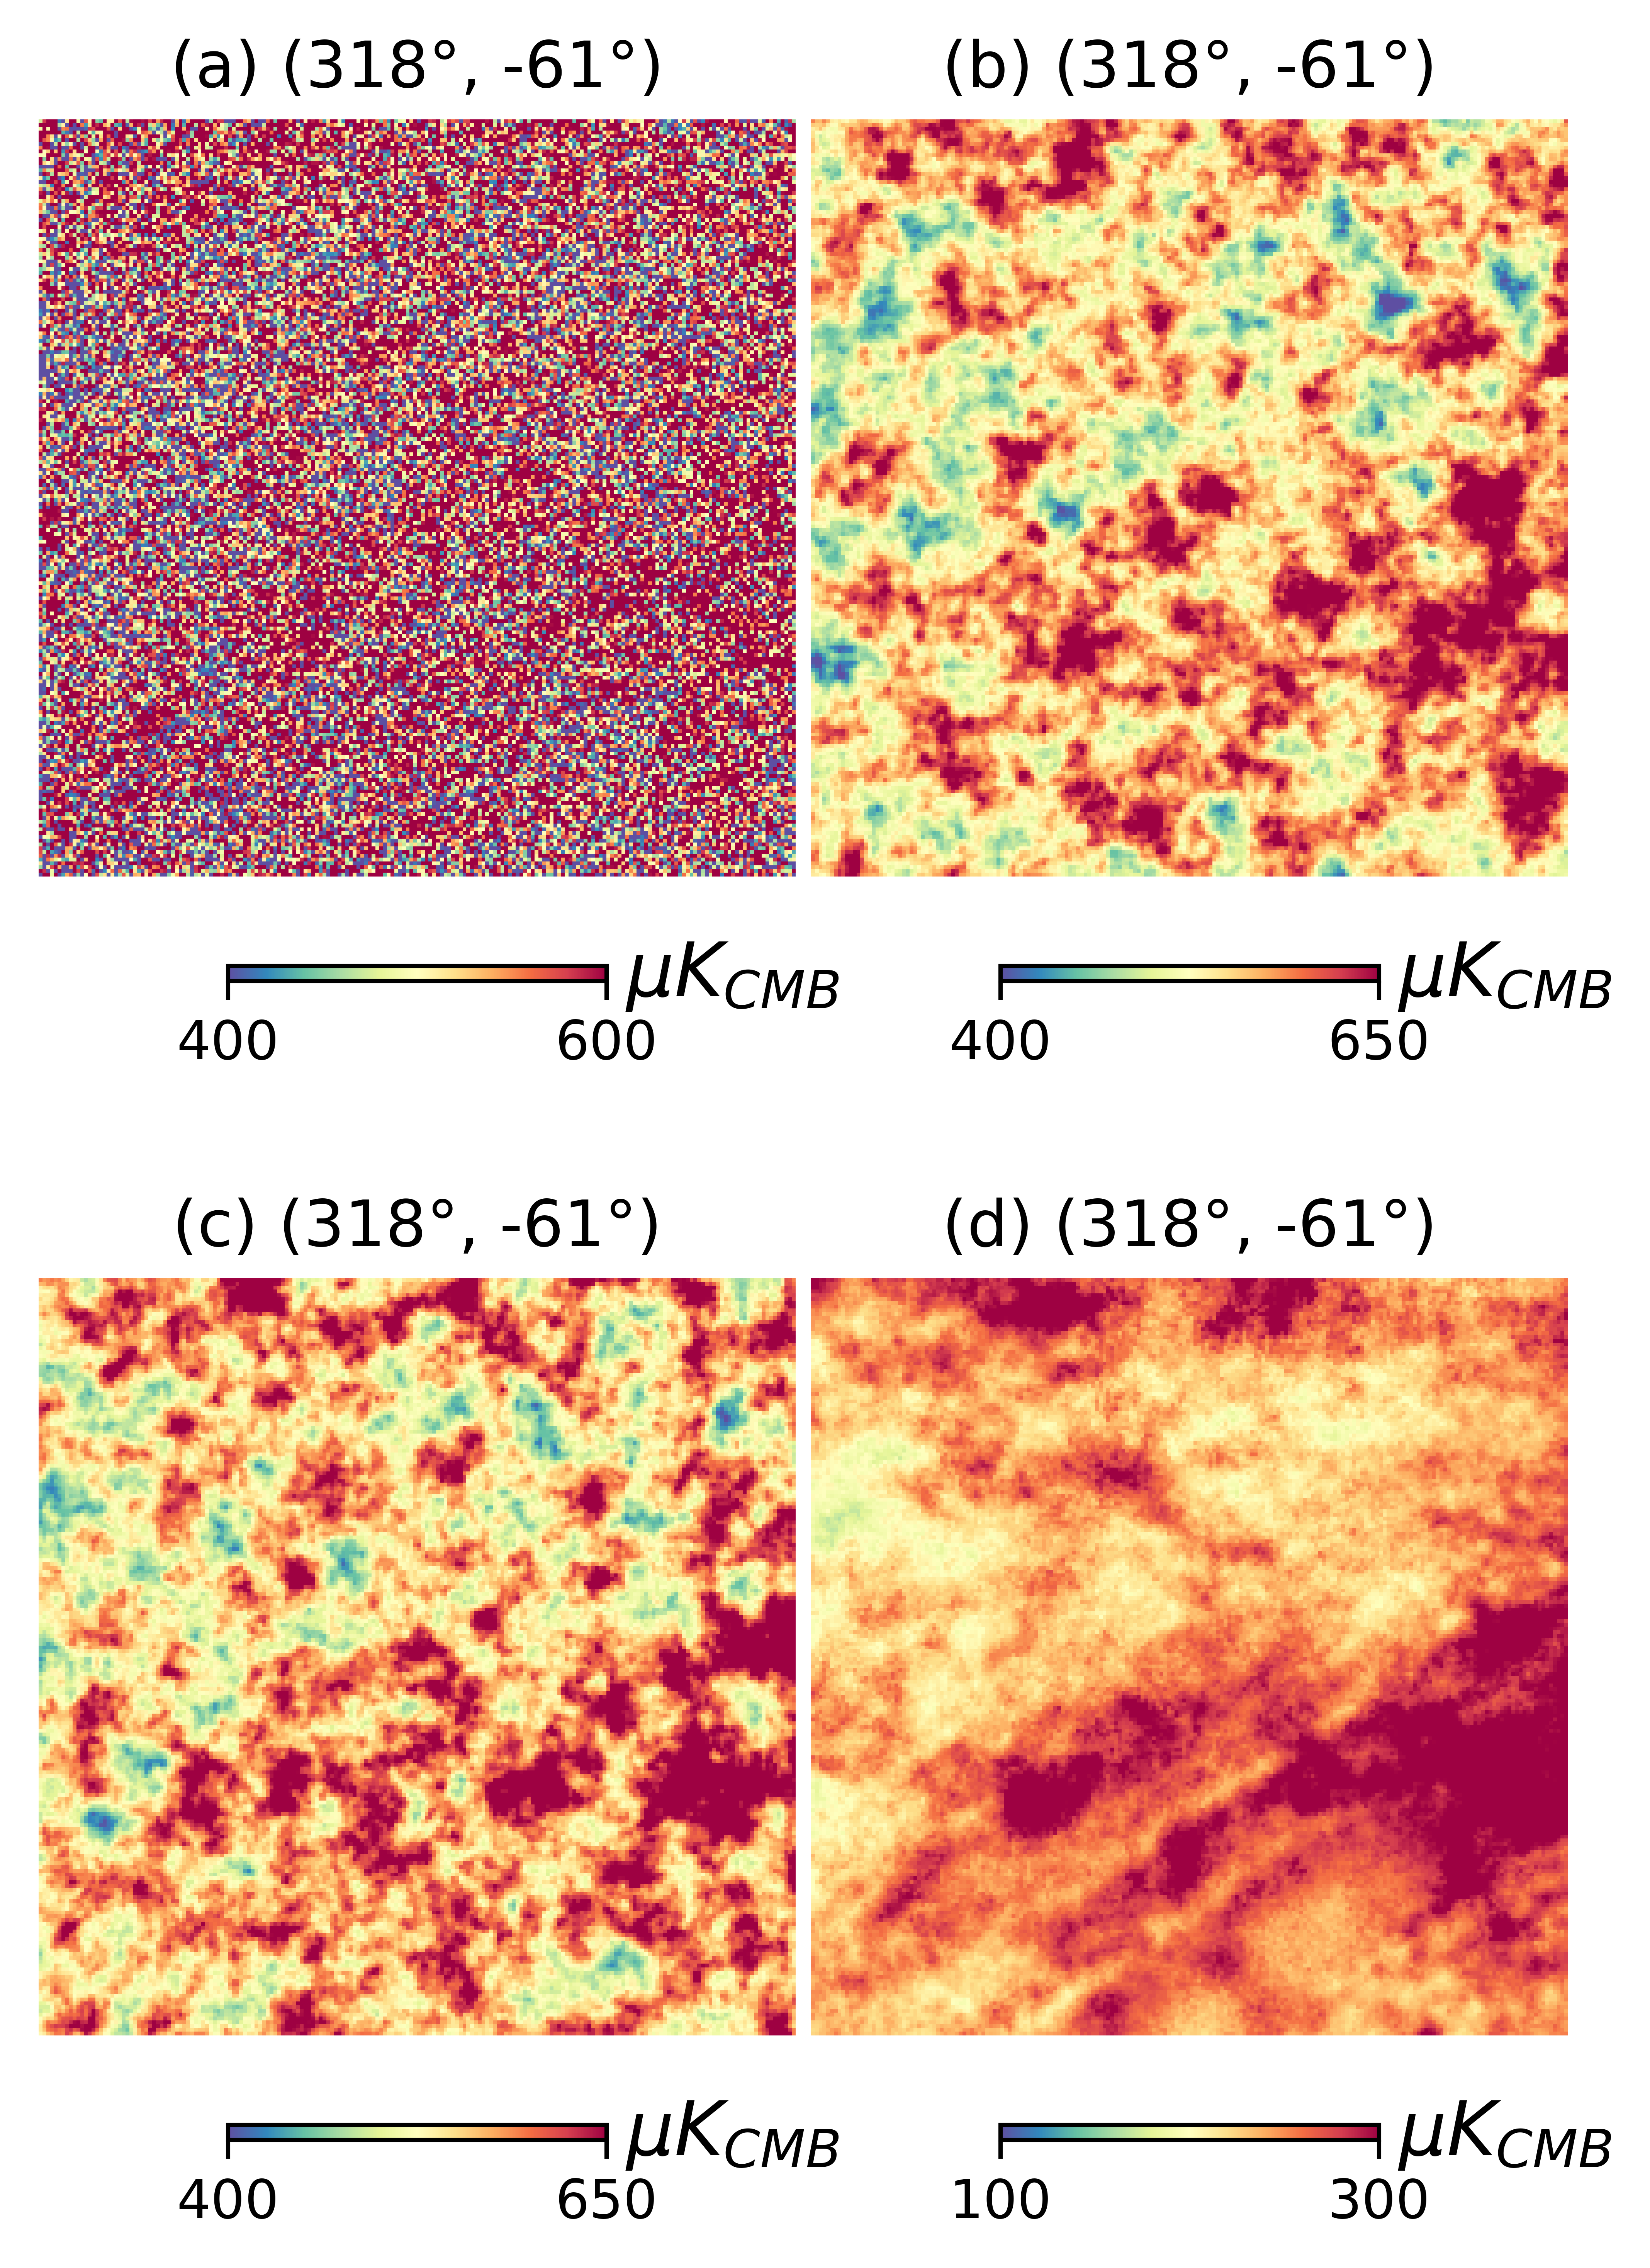
\includegraphics[width=0.48\textwidth]{figures/BK_non_smooth_wo_zero_lvl.png}
    \caption{Dust intensity at 353GHz at [l = 318, b = -61] with an angular resolution of 4.41': (a) PR3 (b) d9 (c) d11 (d) d12\\ Here, PR3 is contaminated by CIB and extragalactic sources.}
    \label{fig:353_int_BK}
\end{figure}

\begin{figure}[ht!]
    \centering
    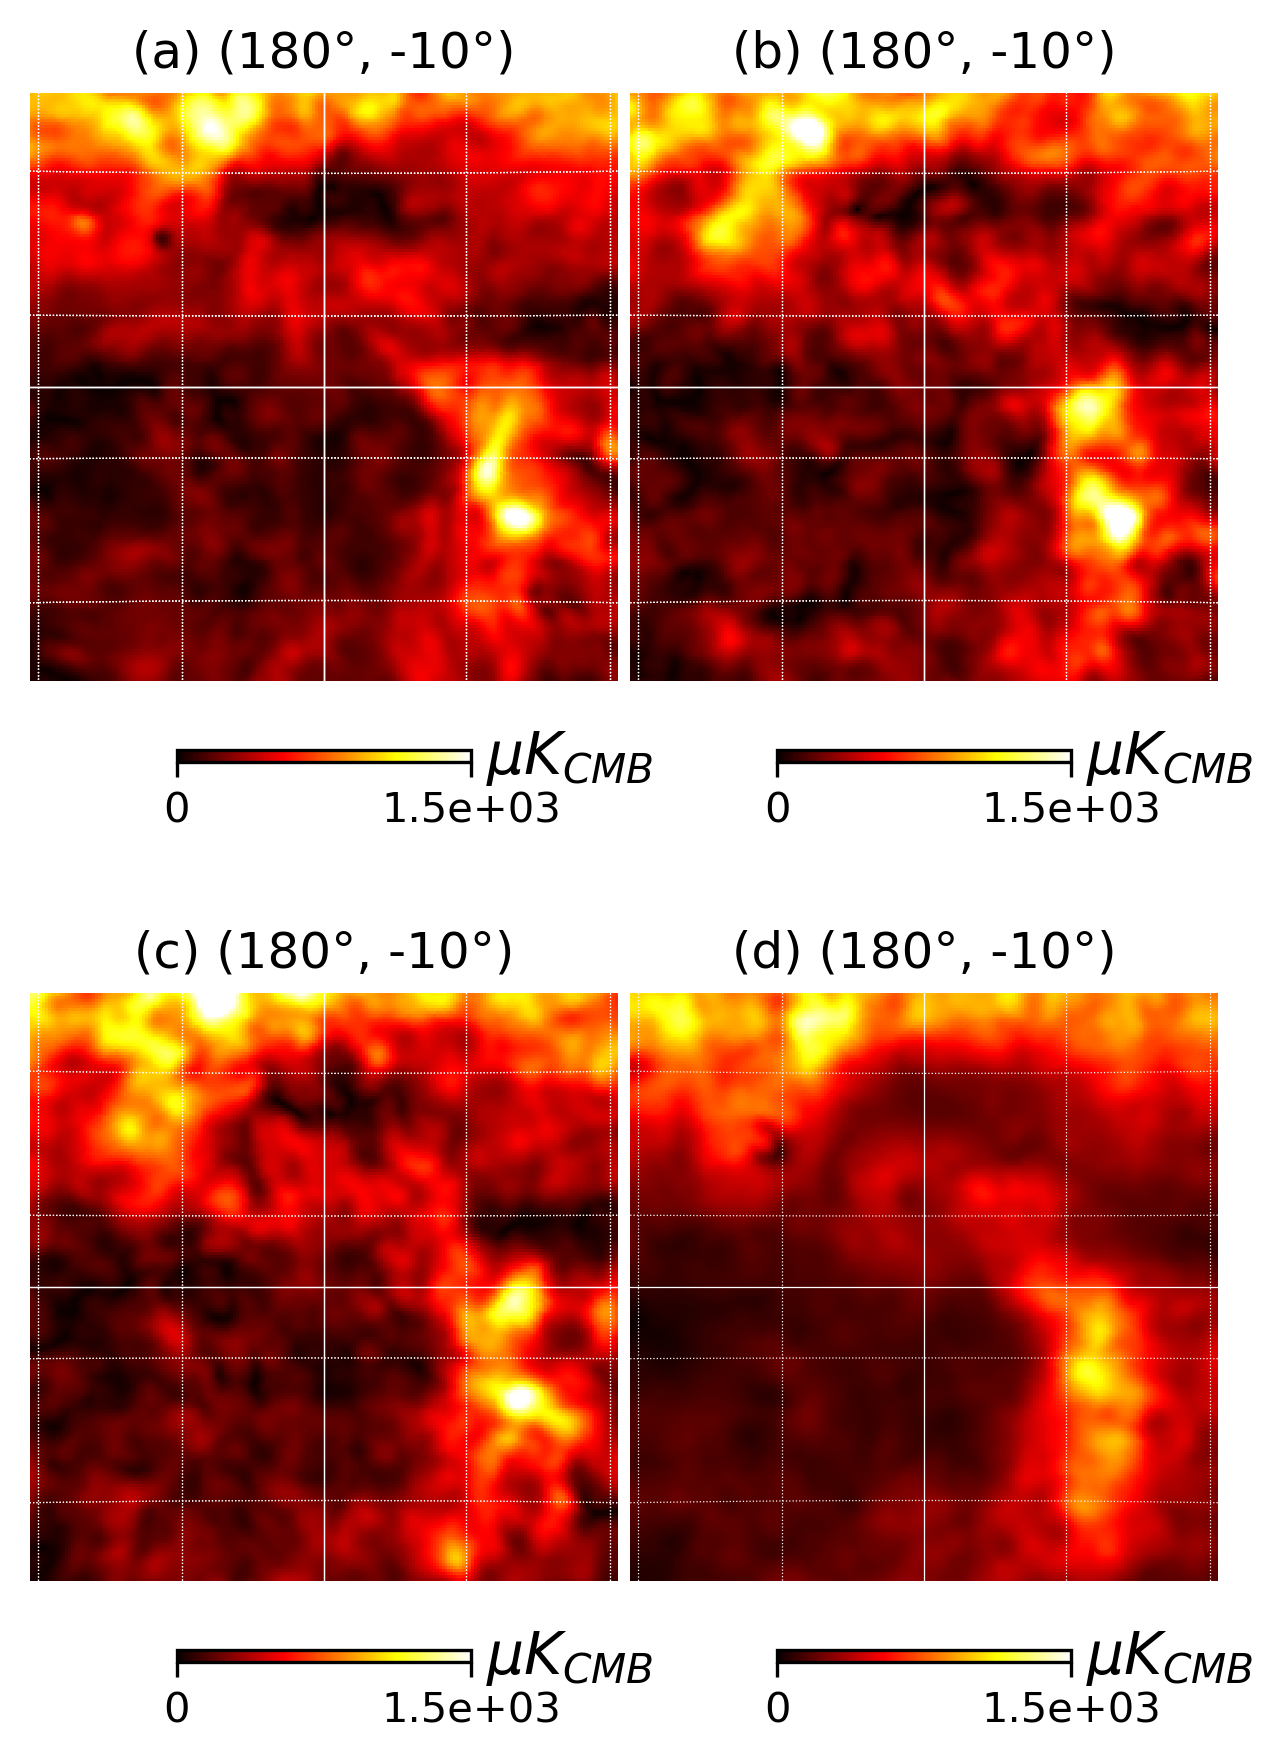
\includegraphics[width=0.48\textwidth]{figures/pol_gal_plane_smooth_30'.png}
    \caption{Polarized dust intensity at 353GHz centered at [l = 180, b = -10] with an angular resolution of 4.41', smoothed to 30 arcmin: (a) PR3 (b) d9 (c) d11 (d) d12.}
    \label{fig:353_pol_int_gal_plane}
\end{figure}
% \begin{figure}
%     \centering
%     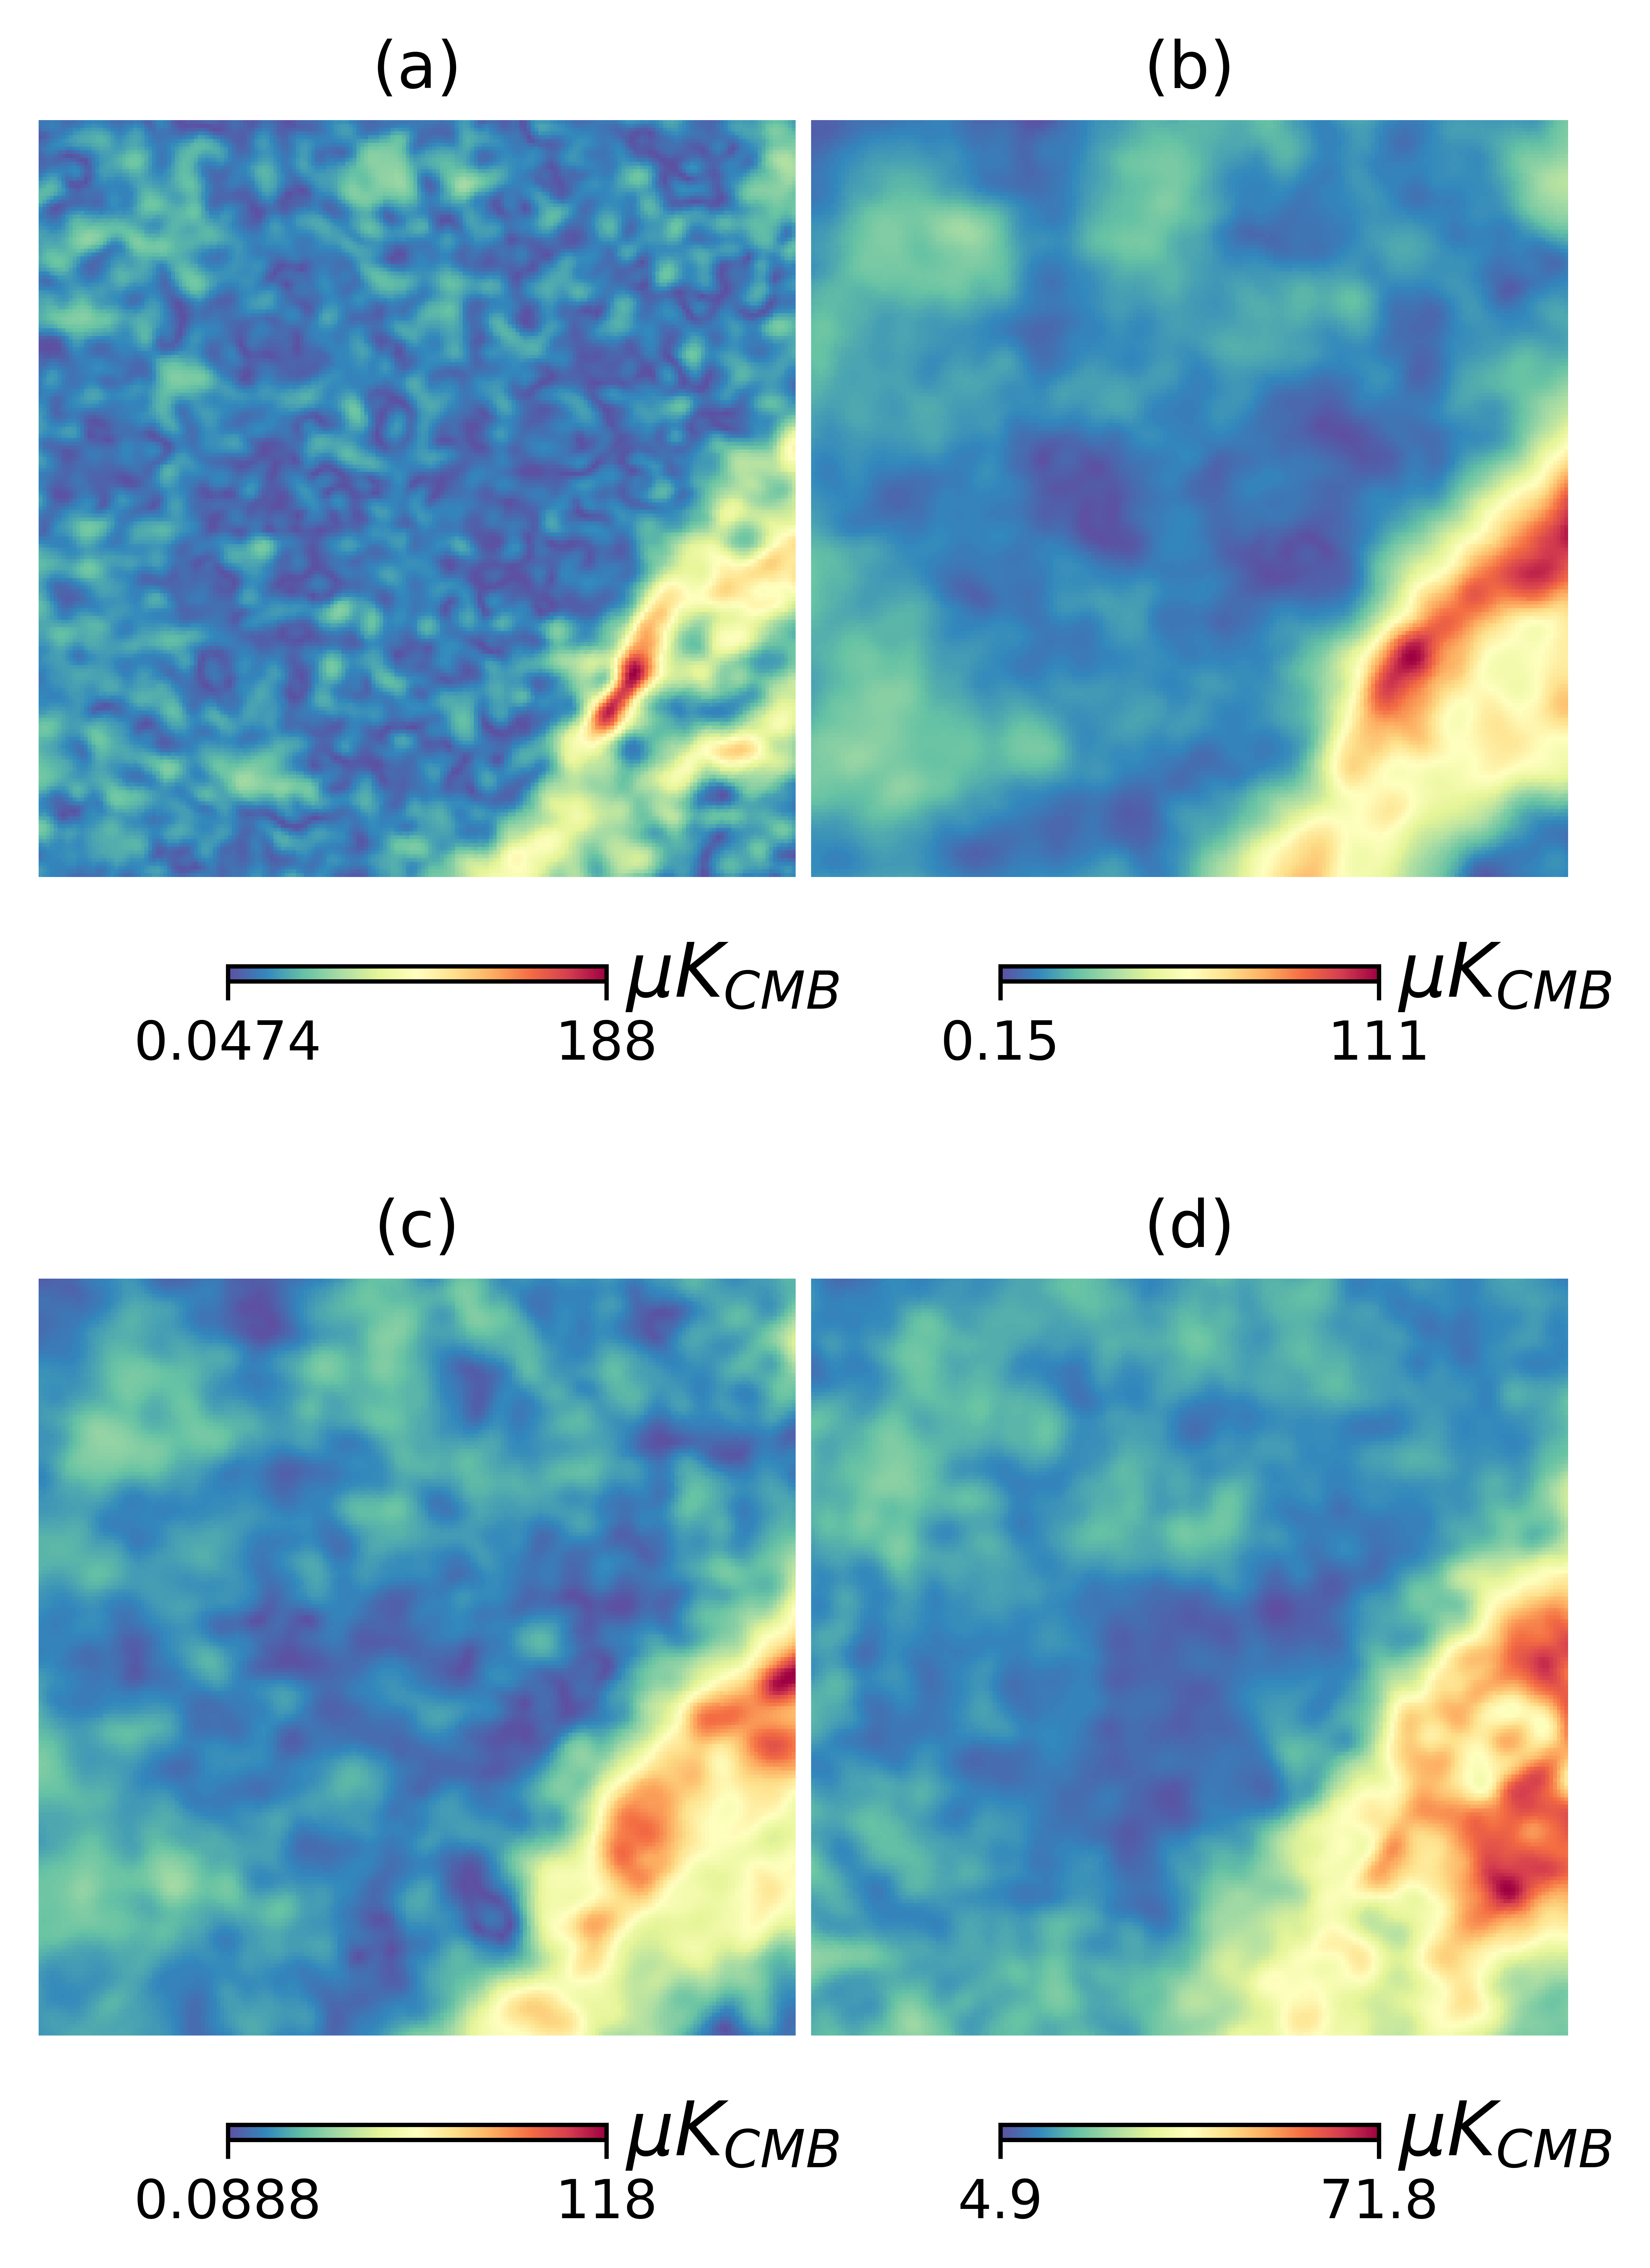
\includegraphics[scale = 0.6]{figures/pol_NGP_smooth_30'.png}
%     \caption{Polarized dust intensity at 353GHz centered at [l = 0, b = 90].}
%     \label{fig:353_pol_int_NGP}
% \end{figure}

\begin{figure}[ht!]
    \centering
    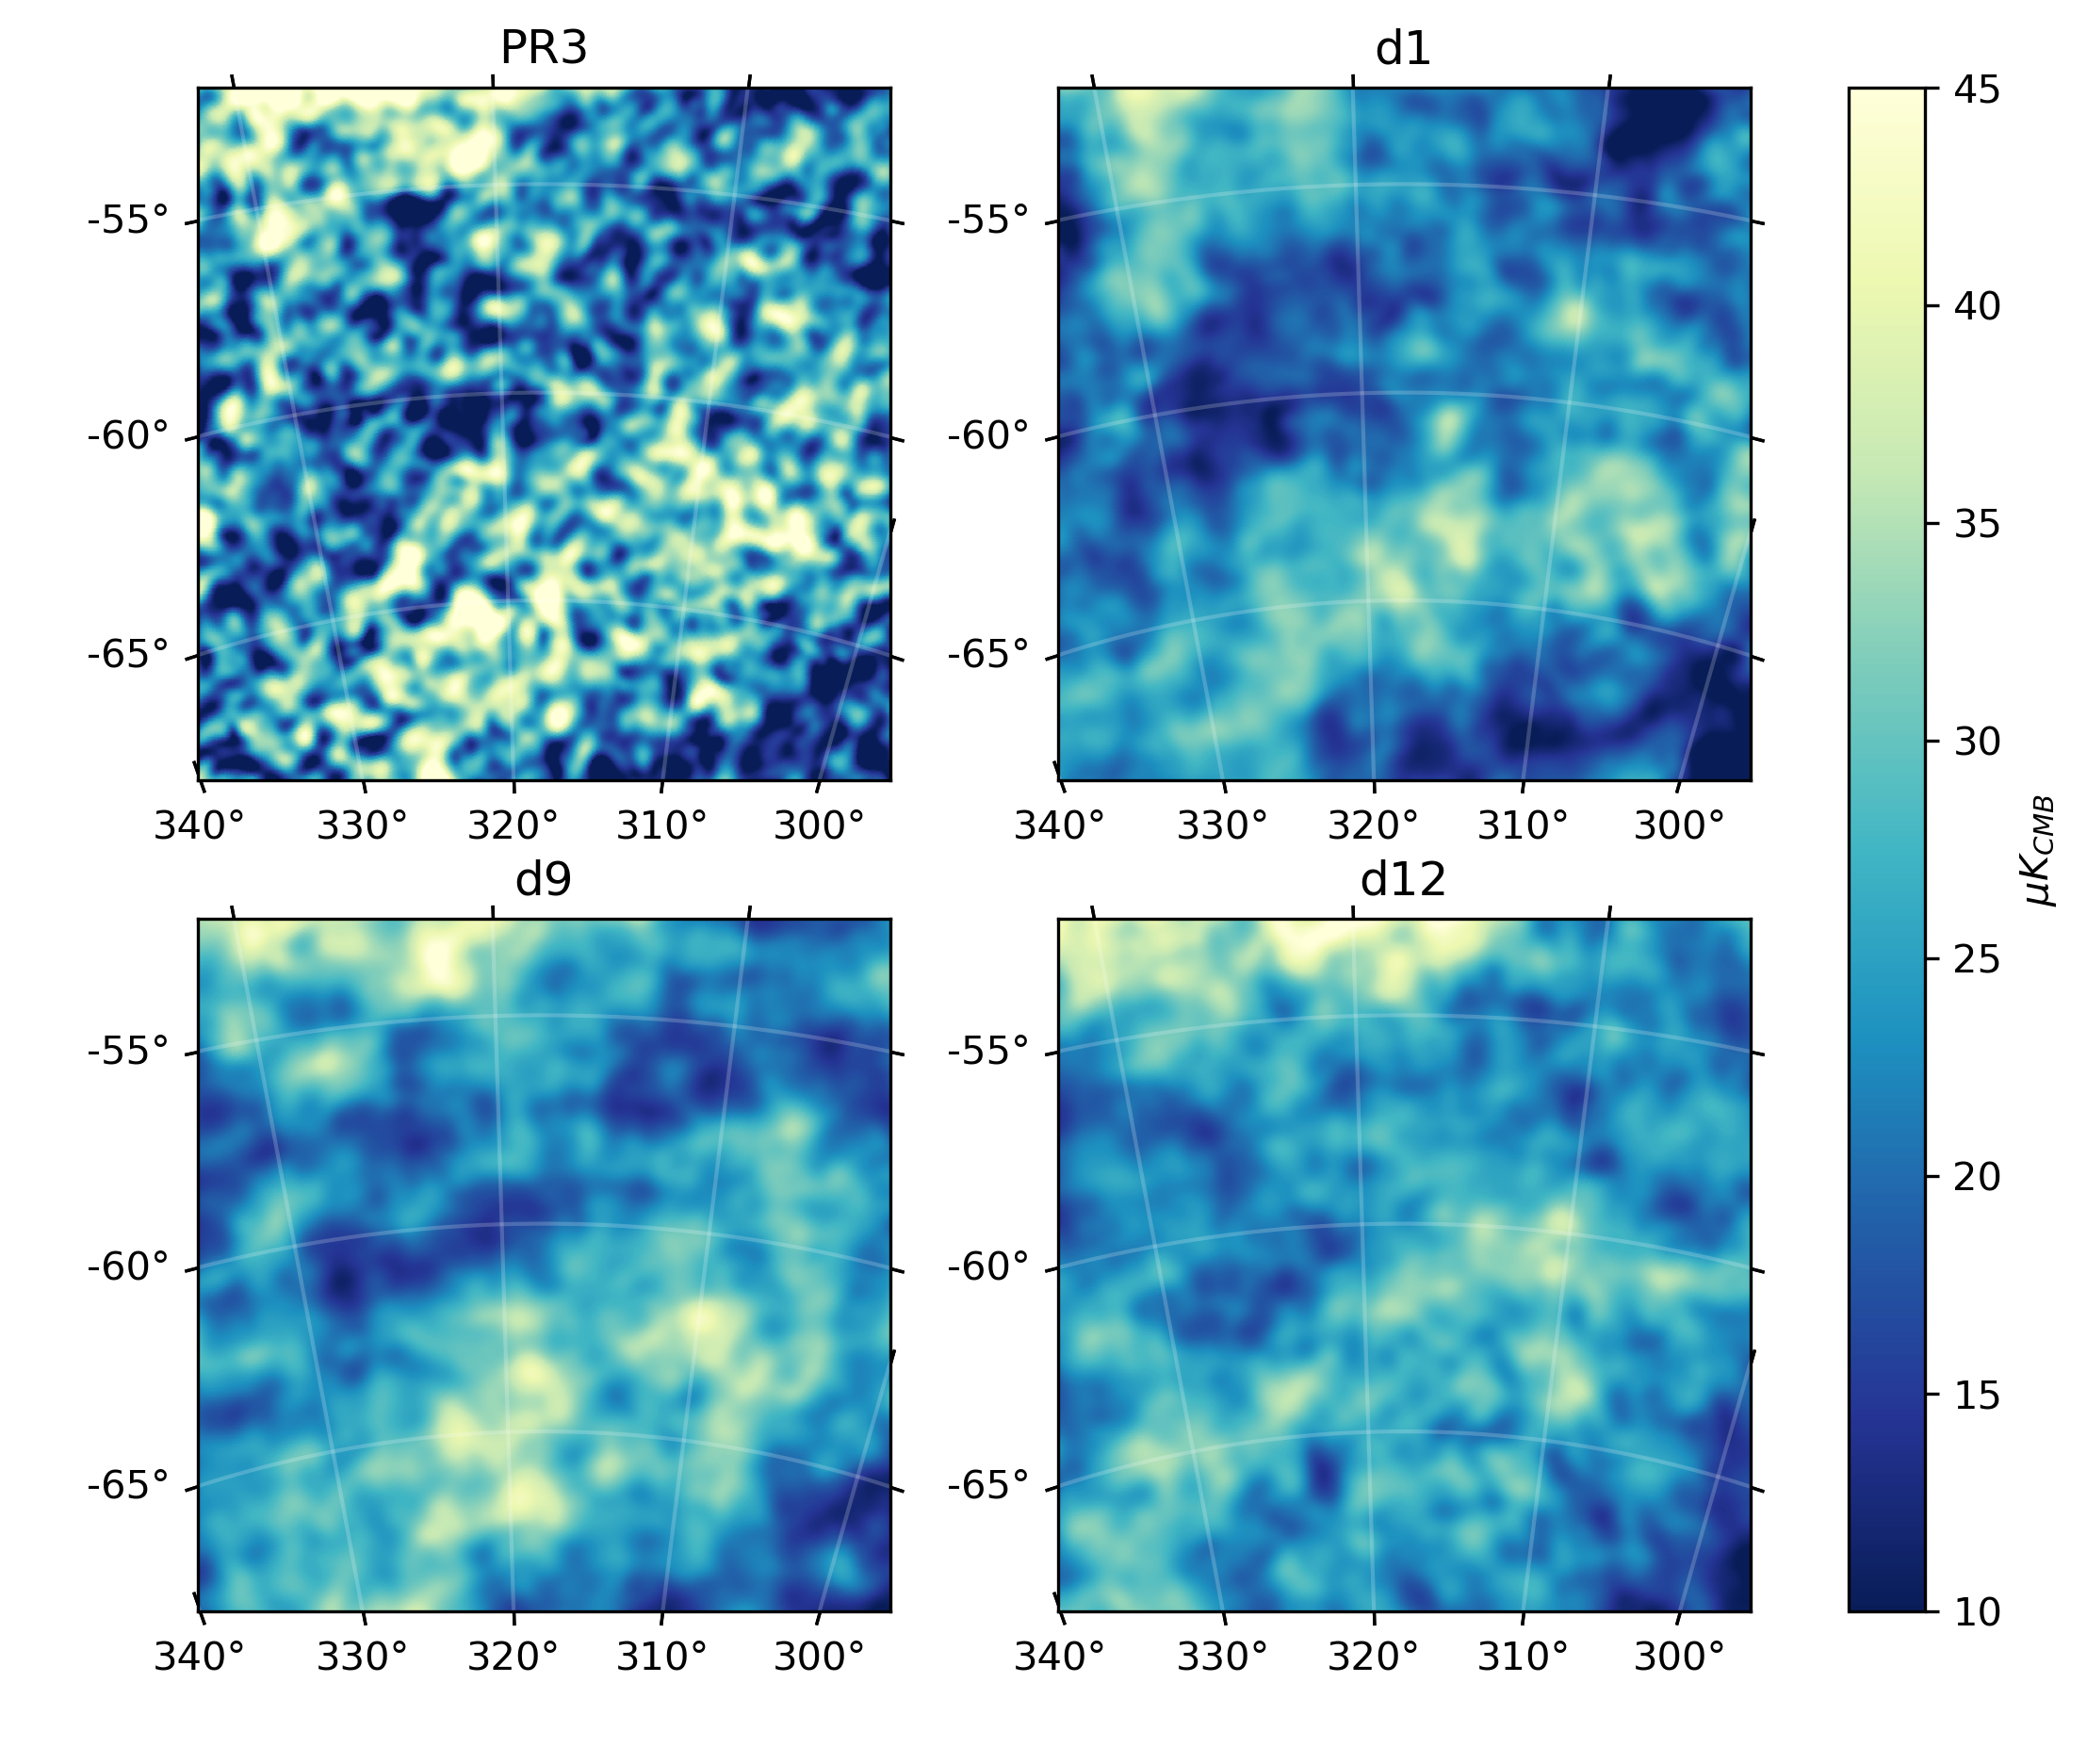
\includegraphics[width=0.48\textwidth]{figures/pol_BK_smooth_30'.png}
    \caption{Polarized dust intensity at 353GHz centered at [l = 318, b = -61] with an angular resolution of 4.41', smoothed to 30 arcmin: (a) PR3 (b) d9 (c) d11 (d) d12.}
    \label{fig:353_pol_int_BK}
\end{figure}

Intensity and polarization at 353~GHz are displayed in Figures~\ref{fig:353_int_gal_plane} to \ref{fig:353_pol_int_BK}. Varying choices for filtering the real data and generation of random small scales result in varying dust emission properties. For Intensity, d9 and d11 are very similar, with a loss of real structures, replaced by random realizations up to a scale of $l_{max} = 16384$, while d12 is more similar to the actual data. 
Around the Bicep / Keck patch center (Figure \ref{fig:353_int_BK}), the PR3 data is contaminated by the CIB, which masks out dust emission. 

For the polarized intensity, close to the Galactic plane (Figure \ref{fig:353_pol_int_gal_plane}), we see a resemblance between the data and the three models. In the North and South poles, noise dominates in PR3 without smoothing, so the comparison is made at a resolution of 30 arcmin. Overall, the agreement seems adequate between the models and the data considering the current level of uncertainties. 
%After smoothing with a Gaussian beam of 30 arcmin, we discern dust structures.


\subsubsection{Decorrelation} \label{sec:decorrelation}

In this section, we compare the decorrelation properties of various models, computed on the Galactic masks of the previous Section. The decorrelation parameter

\begin{equation}
    \mathcal{R}^{XY}_\ell(\nu_1\times\nu_2) = \frac{\mathcal{D}_\ell^{XY}(\nu_1\times\nu_2)}{\sqrt{\mathcal{D}_\ell^{XY}(\nu_1\times\nu_1)\mathcal{D}_\ell^{XY}(\nu_2\times\nu_2)}}
\end{equation}

Myra Norton's decorrelation plot to go here. Github: https://github.com/galsci/pysm/issues/123

\subsection{Extragalactic Contamination} \label{sec:CIBcontamination}

[Stanford student Monica Hicks is working with Susan on cross-correlating our models with galaxy surveys a la Chiang \& Menard. Hopefully summary figure here.] 

%Our Galactic dust templates are based on measurements of the 
We quantify the extragalactic contamination present in our dust models using a tomographic redshift-clustering technique \citep{Schmidt:2015, Chiang:2019}. Our intensity-based Galactic dust templates inevitably contain emission from both Galactic dust and external galaxies. As described in Section \ref{sec:dustamplitude}, the new \texttt{d9} and \texttt{d10} dust templates are derived from GNILC-processed Planck data, while older PySM dust templates used \texttt{Commander} data products. We thus expect that the new Galactic dust models are significantly less affected by CIB contamination than previous models. Here we quantify this contamination by measuring the angular cross-correlation between our dust models and the clustering of galaxies as a function of redshift in spectroscopic survey data. A perfect Galactic dust template would be uncorrelated with such clustering; the signature of CIB contamination is excess template emission correlated with galaxy clustering. 

Following the procedure in \citet{Chiang:2019}, we 


\subsection{Non-Gaussianity} \label{sec:nongaussianity}
writing: Yao + Nico

In this section, we investigate the level of non-Gaussianity induced in the small scales generated through the polarization fraction tensor transformation. We do that by comparing the Minkowski Functionals (MFs) of the small scales structures from this framework with those from Gaussian realizations of extrapolated power law in standard $IQU$ domain, focusing on the thermal dust component.

In particular, for any n-dimensional excursion set defined with a threshold value $\rho$, there exists $n+1$ kinds of MFs that geometrically and topologically describe the morphology of the set \citep{}. These MFs have long been used as estimators of non-Gaussianity. Therefore, in our case, for the 2-dimensional maps, we have 3 kinds of MFs, $\mathcal{V}_0$, $\mathcal{V}_1$ and $\mathcal{V}_2$ which corresponds to the area, the length and the connectivity of the excursion set.

To help determine the extra non-Gaussianity introduced by going into $iqu$ domain, we build a reference set made of 50 Gaussian realizations small scales structures, generated from the power law fitted to the power spectra of the final sets of maps obtained by going into $iqu$ domain, in particular:

\begin{enumerate}

\item we first fit power laws to the $TT$ ($EE$, $BB$) power spectra in the multipole range $[550, 900]$ ($[400, 700]$) obtained from the full sky maps generated through the polarization tensor formalism, and extrapolate them up to $\ell_{\rm max}=4096$. 
\item To generate only the small scales, we apply a high-pass filter to the fitted power law with $\ell_{cut} = 400$ and 110 for intensity and polarization respectively, and then generate full sky small scales realizations using \texttt{synfast}. 
\item These full-sky small scales are then multiplied with modulation maps. 
\item At the same time, the small scales in the real data are filtered out and the large scales remain untouched.
\item At last, the generated Gaussian small scales are added into observed large scales to form the final set of maps. 
\end{enumerate}

Now we have two sets of maps with different small scales co-added: one with small scales generated in $iqu$ domain, the other with modulated Gaussian small scales in the $IQU$ domain. We then apply a high-pass filter to retain only the small scales of these two set of maps, that we call \texttt{poltens-ss} and \texttt{Gaussian-ss}. To calculate the MFs we select several patches on the sky and project them onto flat plane.

Note that the design of the modulation maps is to ensure the final \texttt{Gaussian-ss} maps  have the same power spectra behavior as \texttt{poltens-ss}, on different masks that exclude the inner part of the Galactic plane. 

Here we present the comparison results for two specific patches with centers at [$0^{\circ}$ , $45^{\circ} $] and [$45^{\circ}$ , $45^{\circ} $], each with dimension of $20^{\circ}\times20^{\circ}$,  as shown in Fig.~\ref{fig:maps:patch2} and ~\ref{fig:maps:patch1}.

In Fig.~\ref{fig:MF:patch2} and ~\ref{fig:MF:patch1}, the three MFs for I, Q and U for the two sets of maps are shown, for the two patches considered. The shaded region is the dispersion of MFs over 50 realizations and the solid line is the mean. The blue dotted one is for \texttt{Gaussian-ss} while the orange solid one is from \texttt{poltens-ss}.

We can see that in Figure~\ref{fig:MF:patch2} for the patch with center [$45^{\circ}$ , $45^{\circ} $], the mean values and dispersions of the MFs of \texttt{poltens-ss} and \texttt{Gaussian-ss} are highly overlapped with each other, which means that in this patch the generation of maps in $iqu$ domain does not lead to any extra non-Gaussian structure. While in Fig.~\ref{fig:MF:patch1} for the patch [$0^{\circ}$ , $45^{\circ} $], a significant difference is visible between the MFs of \texttt{poltens-ss} and \texttt{Gaussian-ss} which indicates the difference in the level of non-Gaussianity in \texttt{poltens-ss} and \texttt{Gaussian-ss}. By looking into the details of Figure~\ref{fig:maps:patch1}, we find the that in this patch there is a strong point source in the intensity map(at [$4.5^{\circ}$ , $36.5^{\circ} $]) which leak power into the polarization map through the polarization tensor transformation. However in the Gaussian small scales there will not be such leakage from the point source.  

The two patches shown in Fig.~\ref{fig:MF:patch2} and ~\ref{fig:MF:patch1} are in fact two typical cases of the MFs for different patches considered. In one case the MFs of the two sets of small scales are similar and in the other case the two differs a lot. So overall the \texttt{poltens-ss} will have more non-Gaussianity than \texttt{Gaussian-ss} but this statement depends on the sky position interested. 

\begin{figure*}[hbt]
    \centering
    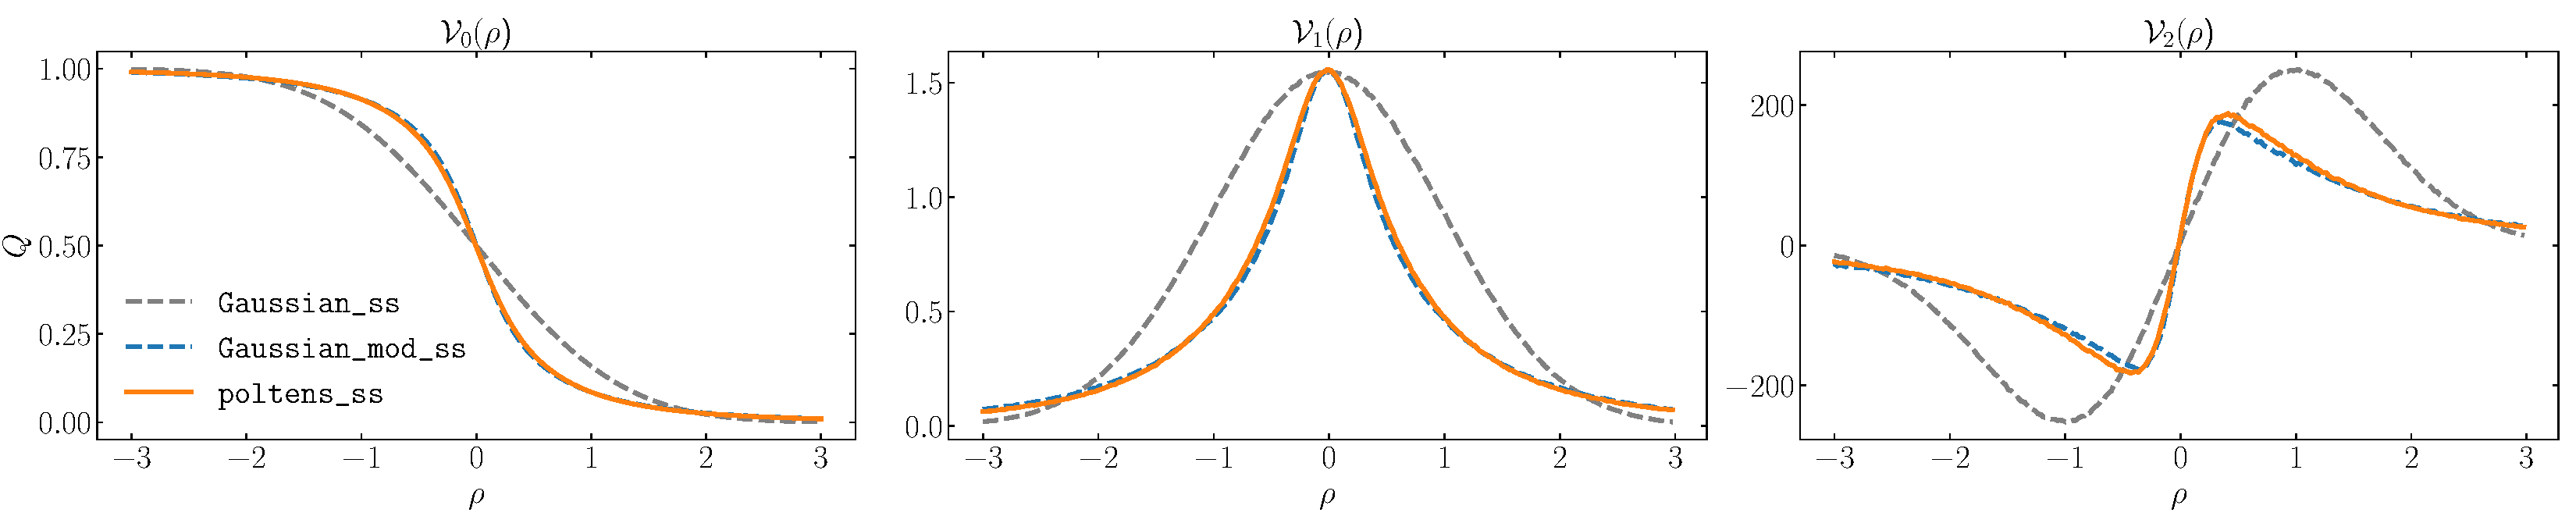
\includegraphics[width=180mm]{figures/MFs_80p_sky_Q.pdf}
    \caption{MFs for the maps on the sphere with 80\% mask. }
    \label{fig:MF:patch1}
\end{figure*}

\begin{figure*}[hbt]
    \centering
    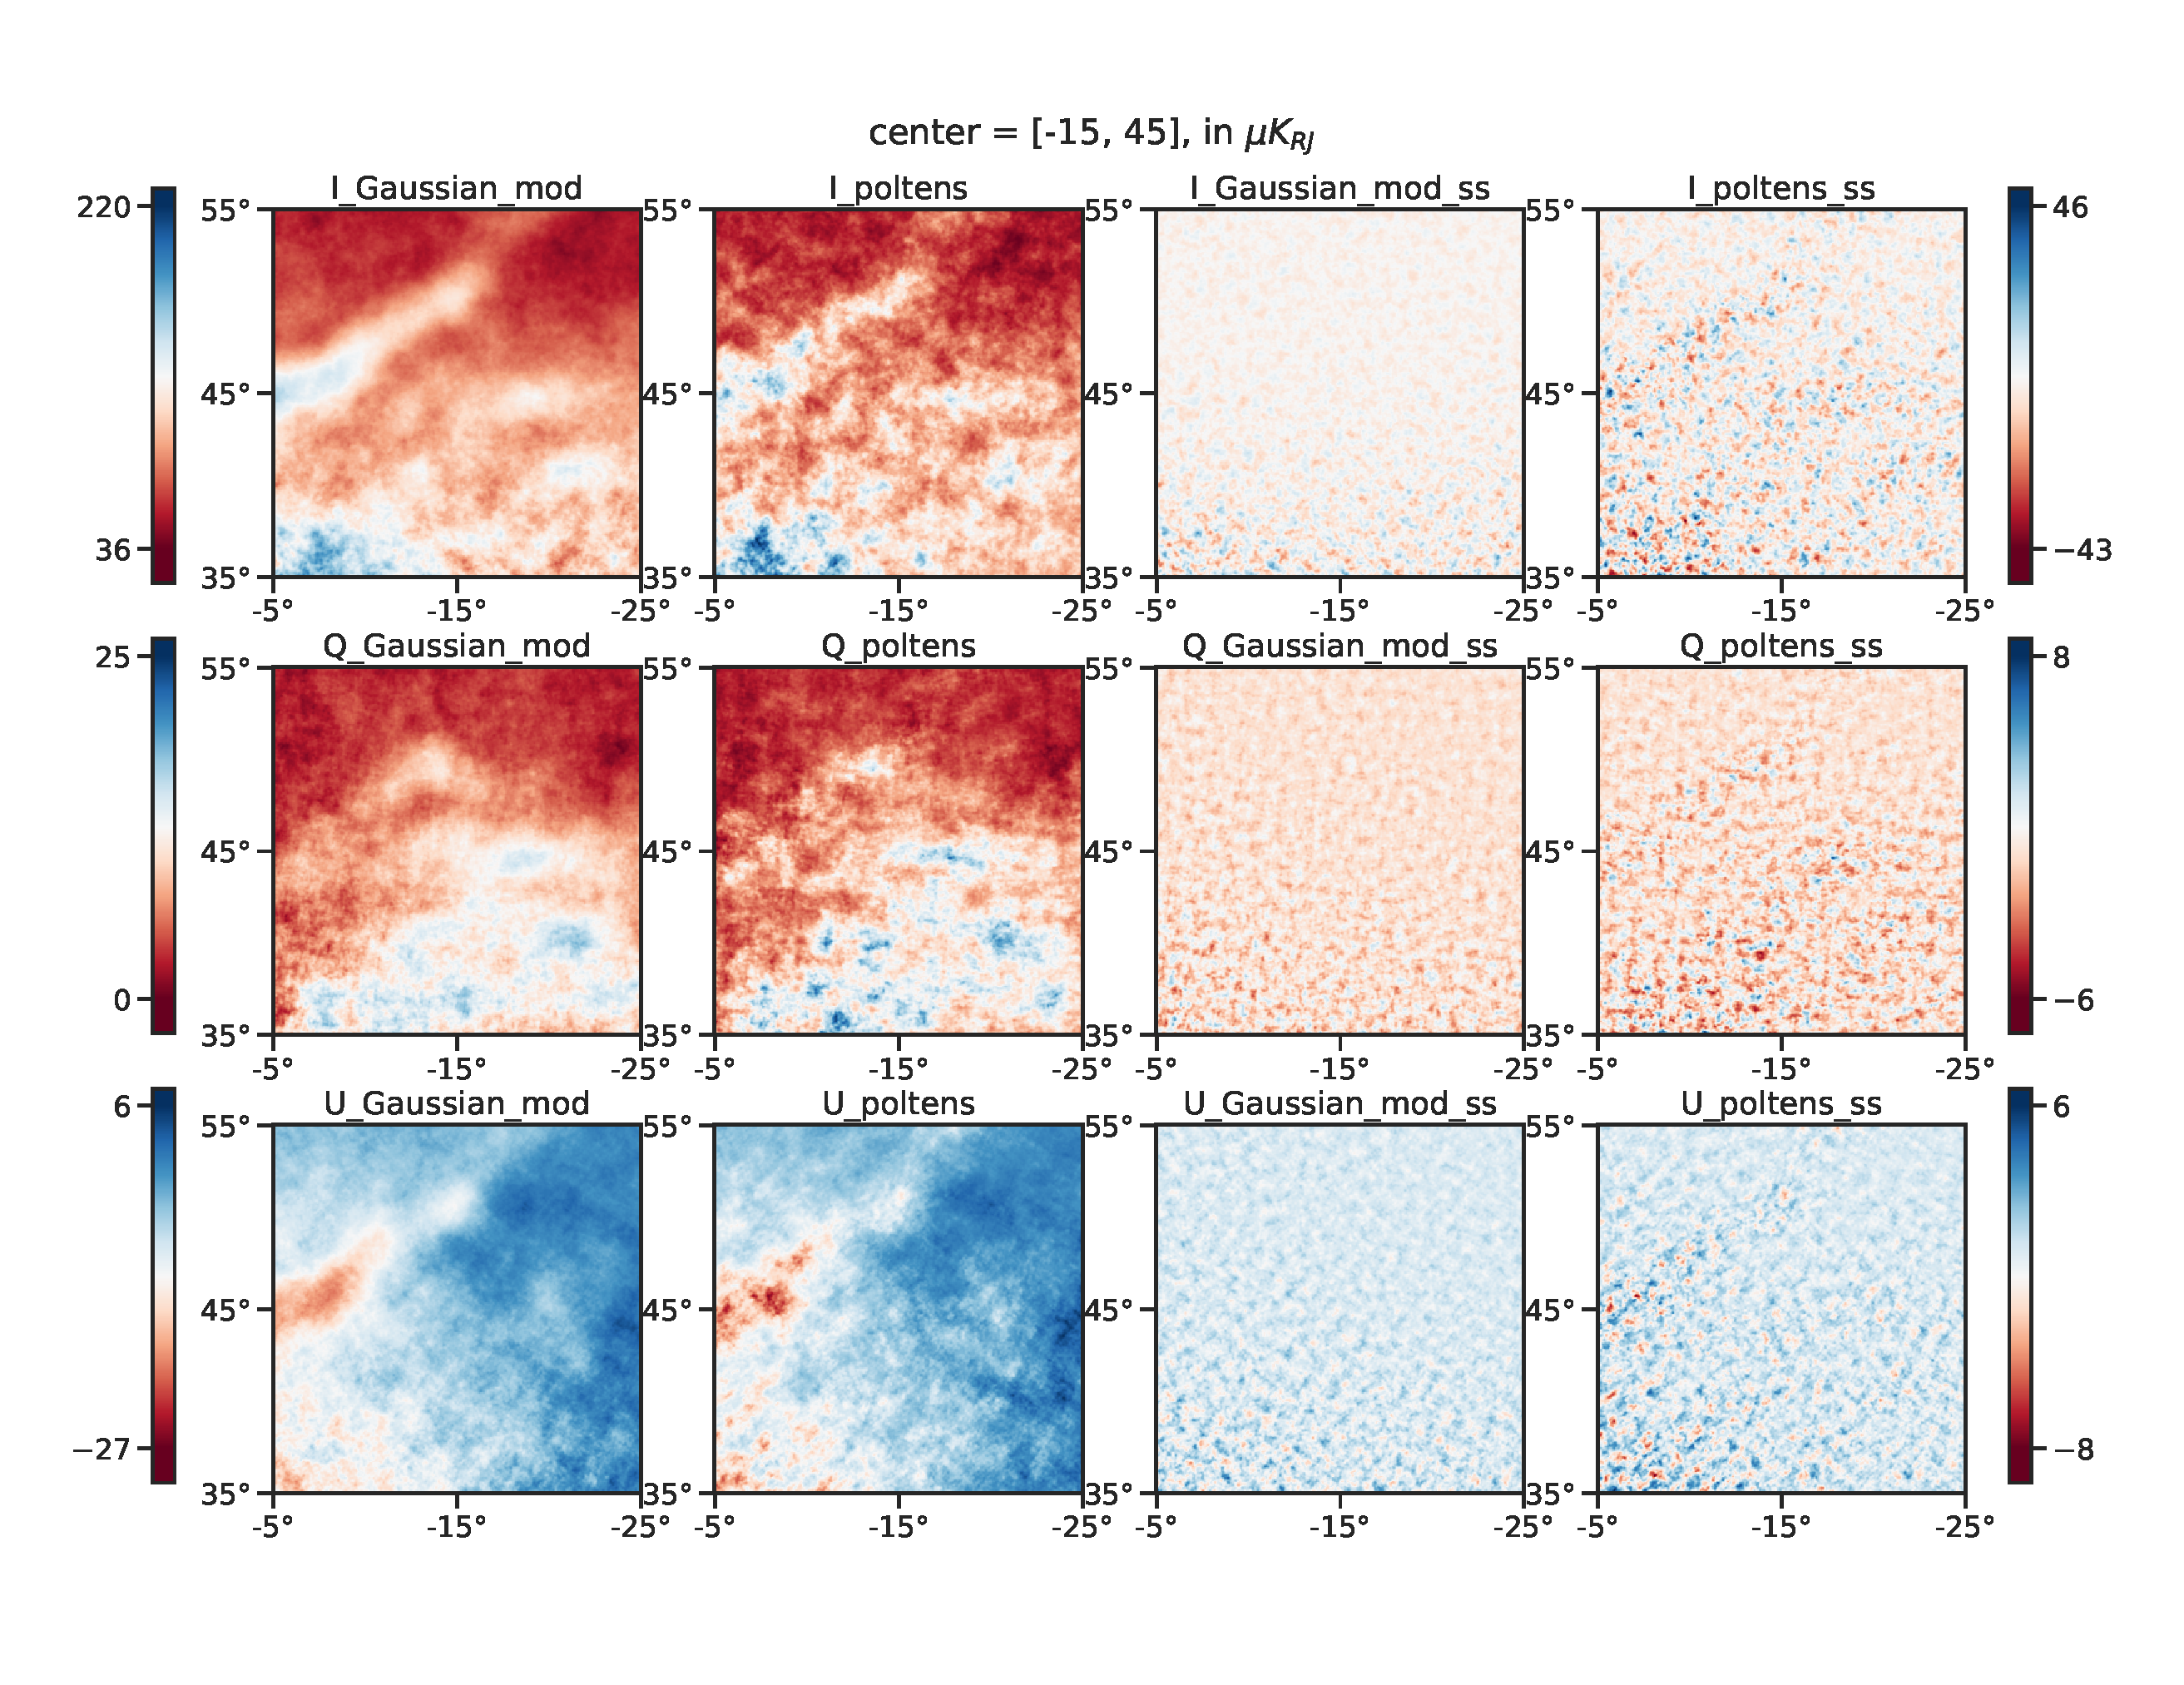
\includegraphics[width=180mm]{figures/maps_patch_345_35.pdf}
    \caption{The zoom-in plot of the maps, in the selected patch with center [$-15^{\circ}$ , $45^{\circ} $]. From left to right, we show the final map with \texttt{Gaussian-mod-ss}, final map with \texttt{poltens-ss}, \texttt{Gaussian-mod-ss} only map and \texttt{poltens-ss} only map. From top to bottom is for I, Q and U respectively. The colorbar on the left indicates the pixel value in the left-most two columns in the units of $\mu K_{RJ}$ and the colorbar on the right is for the last two columns. }
    \label{fig:maps:patch2}
\end{figure*}
\begin{figure*}[hbt]
    \centering
    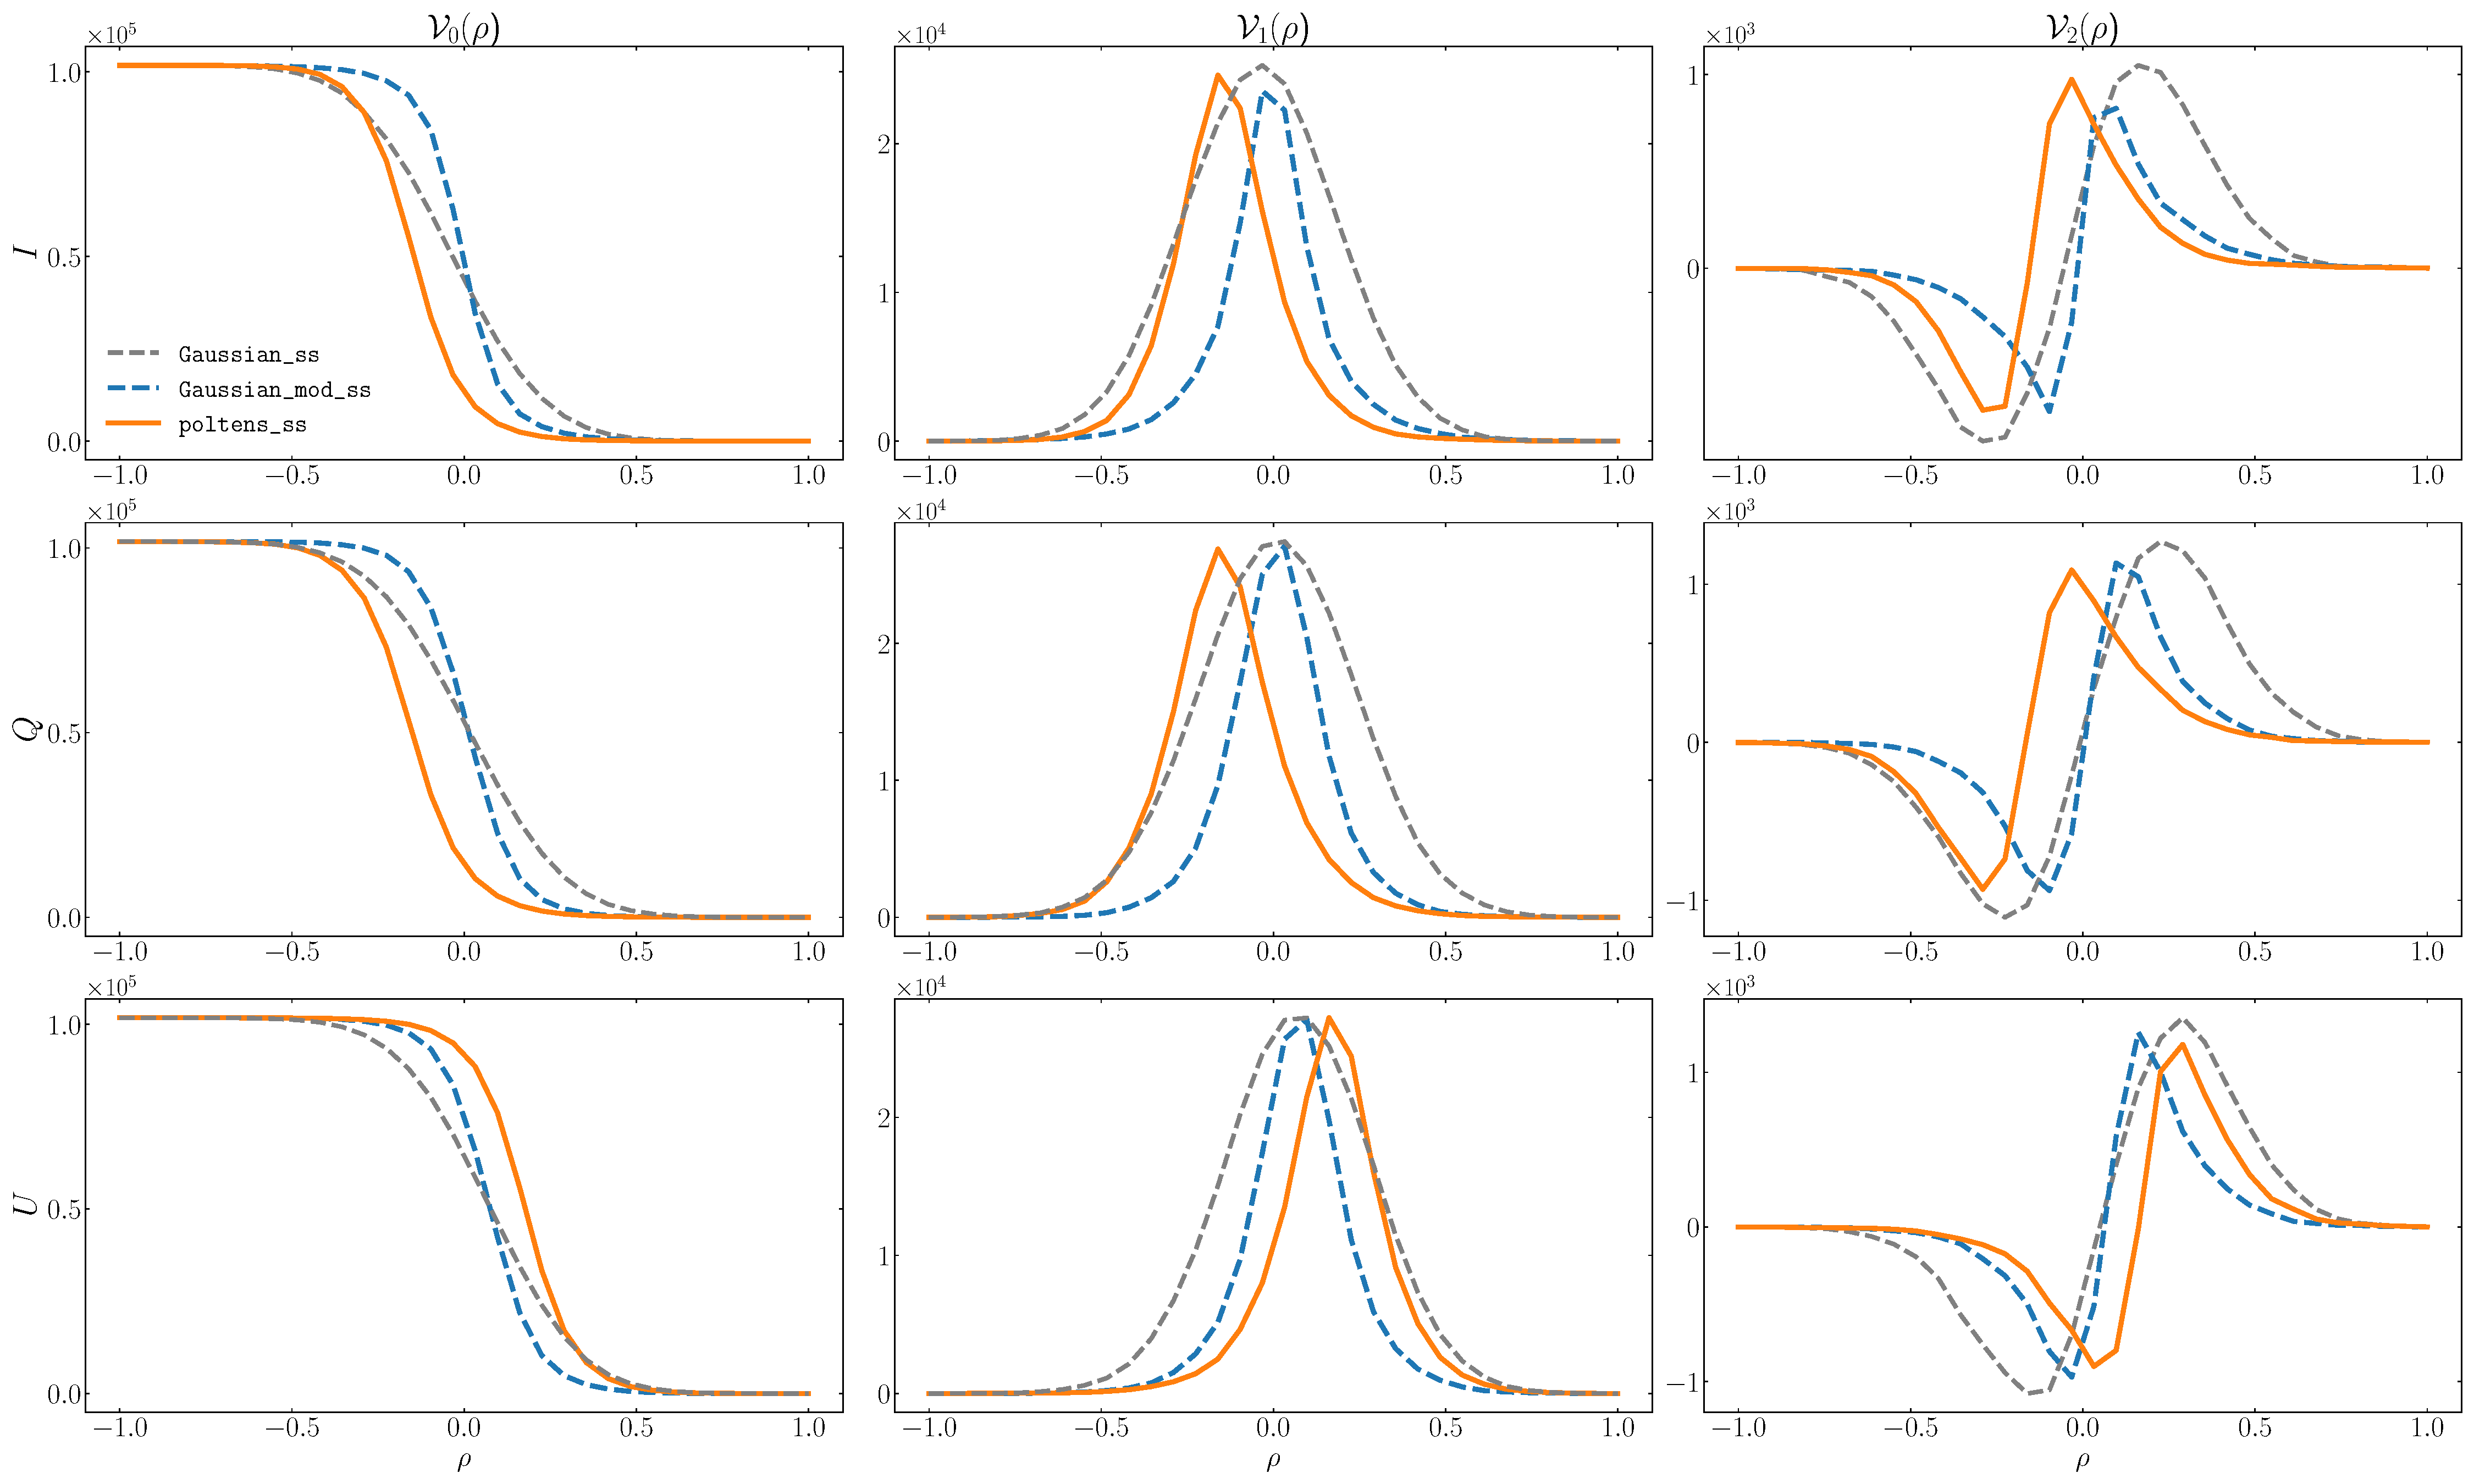
\includegraphics[width=180mm]{figures/MFs_345_45_with_G_rescaled.pdf}
    \caption{Minkowski Functionals as a function of the threshold $\rho$ for the one realization of I, Q and U small scales in the patch with center of [$-15^{\circ}$ , $45^{\circ} $] in Galactic coordinates. Each row shows three kinds of Minkowski Functionals. The blue dotted one is for \texttt{Gaussian-mod-ss} while the orange solid one is from \texttt{poltens-ss}. We also show the \texttt{Gaussian-ss} in dashed gray line as a comparison.}
    \label{fig:MF:patch2}
\end{figure*}


\section{Model Suite}\label{sec:modelsuite}
Writing: Susan + others
\begin{table*}[]
    \centering
    \begin{tabular}{lcc}
    
    \toprule 
    Complexity & Model set & Short description \\
    \midrule
    Low  & \texttt{d9, s4, f1, a1, co1} & sdf  \\
    Medium  & \texttt{d10, s5, f1, a1, co3} & sdf   \\
    High  & \texttt{d12, s7, f1, a2, co3} & MKD dust layer model, spatially varying synchrotron curvature, polarized AME  \\
   
   \bottomrule
    \end{tabular}
    \caption{Summary of the suite of model sets described in Section \ref{sec:modelsuite}. These are recommended combinations of models at three levels of complexity (low, medium, and high).  }
    \label{tab:modelsuite}
\end{table*}

The models available for each emission component can be used in various combinations to form a number of unique Galactic sky models. While every user has this combinatoric freedom, we also prescribe a suite of recommended model sets. Table \ref{tab:modelsuite} details three model sets, representing increasing levels of complexity. The low complexity model set is highly idealized.
The medium complexity model set includes Galactic emission properties that are both expected physically and confirmed observationally, like ..
The high complexity model set models Galactic emission properties that are physically realistic but as-yet undetected, like polarized AME and spatially varying synchrotron curvature. The high complexity model set uses the MKD layer model for Galactic dust emission, and the decorrelation is near the maximum allowed by current constraints.  

%Susan: Either here or before validation, we should have a succinct section that lays out the 3 complexity levels

[Moved from intro, work this in here:]
for example analyzing CMB-S4 data together with that of the precursor South Pole and/or Simons Observatories, or using CMB-S4 high resolution data to help delens LiteBIRD and LiteBIRD high frequency data to help remove dust from CMB-S4.


\section{Discussion} \label{sec:discussion}
writing: Susan + others

\begin{enumerate}
    \item Highlight improvements made and why they are relevant to various CMB science cases
    \item Identify areas where algorithms can be improved (notably modulation of small scales, non-trivial TB/EB correlations)
\end{enumerate}

Susan:
One area for future development is in the implementation of parity-odd polarization quantities ($TB$, $EB$), or effects that give rise to them. The \textit{Planck} 353 GHz data show a positive $TB$ correlation over large angular scales (cite Planck++), and (misalignment, cite Clark/Huffenberger/Cukierman, state importance for CB++)


\section{Summary and Conclusions} \label{sec:summary}

We have done X. The principal conclusions of this work are as follows:

\begin{enumerate}
    \item Some nice bullets here
\end{enumerate}

Short forward-looking paragraph.

\bibliography{refs.bib,refsADS.bib,refsPlanck.bib}

\end{document}
